\chapter{Results}

\label{ch:results}

Tak jak w methodology, trzeba ustalic czy nazywac sekcje metodami (local maxima, odporne selektory, two-stage method, PAR) czy problemami (t-f map enhancement, selection of IFB, significance levels of selectors for filtering purposes, more than 1 damage, frequency modulation due to time-varying load)

W ponizszych sekcjach beda porownania z dotychczasowymi metodami

\section{Time-frequency map enhancement - skompilowac z Ferrara}\label{methodology_tf_enh}

In this section we present in details  the local maxima method which was previously based on non-overlapping windows in short time Fourier transform~\cite{Obuchowski2014325}. Here we describe how to adapt it to highly-overlapping windows.\\
The local maxima method starts with a transformation which converts a signal in time domain into a two-dimensional map (time-frequency), where spikes in time domain become wide-band excitations. In this paper we use the short-time Fourier transform that is denoted by $\{STFT(t,f)\}_{t\in T, f\in F}$, where $T$ is the set of time points and $F$ stands for the set of frequencies for which the transform is calculated. In the further analysis we assume $T=\{t_1,....,t_{\#T}\}$, where $\#T$ denotes number of elements of the set $T$. The STFT for random sample $X_1, ...,X_n$, time point $t_i$ and frequency $f$ is defined as follows:
\begin{eqnarray}
STFT(t_i,f)=\sum_{k=1}^{n}X_k\tilde{W}_{k-t_i}e^{jfk},
\end{eqnarray}
where $\{\tilde{W}_k\}$ is the window sequence.\\
Once the map is obtained, time series related to each $f\in F$ are analyzed.  For a given $f\in F$  and $t_i$ we put $M(t_i,f)=1$ if $|STFT(t_i,f)|=max\{|STFT(t_k,f)|: i-r\leq k\leq i+r\}$ and $M(t_i,f)=0$ elsewhere. The binary spectrogram obtained by applying this rule for every time series should have clearly visible wide-band excitations with small amount of local maxima between them if $r$ is properly chosen. We suggest  that $r$ (called the minimal neighborhood length) should be as high as it is possible to theoretically preserve all the cyclic wide-band excitations related to damage in a rotating machine. In the non-overlapping windows case $r$ is calculated as the highest integer value not greater than ratio of the expected time between the following disturbances to the STFT window length, both expressed in the same units, i.e. in samples or in a unit of time. The formula for $r$ is:
\begin{eqnarray}r=\left\lfloor (fs/ff)/Nw-1\right\rfloor\label{tf_enh_row1}
\end{eqnarray}
where $fs$ is the sampling frequency, $ff$ is the fault frequency, $Nw$ stands for the STFT window length and $\lfloor x\rfloor$ is the largest integer not greater than $x$. In the overlapping windows case we propose to modify equation (\ref{tf_enh_row1}) as follows:
\begin{eqnarray}\label{tf_enh_row2}
r=\left\lfloor ((fs/ff)/Nw-1)/(1-Ov)\right\rfloor,
\end{eqnarray}
where $Ov$ denotes overlap ratio, i.e. the ratio of the number of samples that each window overlaps to the window length. In the further analysis we use $Ov=0.95$ and compare it to $Ov=0$. In practice, there might be some deviations from the theoretical distance between local maxima. To illustrate this point, consider series of impulses of different height. It can be caused both by random character of shocks and random background noise. Relaxation of the impulses, even in local damage case, takes a little of time so the real distance between local maxima in a particular time series might be a little smaller than theoretical. Moreover, some of rotating machines exhibit jitter (e.g. bearings) during operation under constant rotational speed, so the real distance might be a little higher or lower than the distance obtained by using equation (\ref{tf_enh_row2}).\\
The next step in our procedure is to calculate the vector of weights and combine it with the binary spectrogram obtaining the enhanced spectrogram. The latter one is formulated as follows:
\begin{eqnarray}\label{tf_enh_row3}
ENH(t_i,f)=W(t_i)M(t_i,f),
\end{eqnarray}
where $W(t_i)=\frac{1}{\#F}\sum_{f\in F}M(t_i,f)$ is the vector of weights and $M(t_i,f)$  represents binary valued time series of the local maxima occurrence
for a time point  $t_i$ and frequency $f$. Conversion of the time-frequency map $\{|STFT(t,f)|\}_{t\in T, f\in F}$ into the binary matrix $\{M(t,f)\}_{t\in T, f\in F}$ preserves energy-invariance, i.e. local maxima in a low-energy frequency bin are as significant as local maxima in other frequency bin. An impulse in the vector of weights calculated as average value of $\{M(t_i,f)\}_{f\in F}$, for a particular time $t_i$ is present only if there is a significant number of local maxima at $t_i$, i.e. larger than in the case where local maxima at $t_i$ are the result of random character of the signal. If there are no wideband exciatations in the time-frequency map or frequency bands of the excitations are not significantly wide then the vector of weights has no pulses. Thus, in locally damaged machine case the enhanced time frequency map increases visibility of wideband excitations and decreases influence of high-energy components. In healthy machine case it presents time-frequency map without any pattern. Moreover, arithmetic mean in the formula for $W(t_i)$ makes the result invariant to number of points at which FFT is calculated.\\
In the next step of our procedure we propose to analyze the enhanced version of vector of weights, i.e. vector calculated as follows:
\begin{eqnarray}\label{tf_enh_row4}
V(t_i)=\frac{1}{\#F}\sum_{f\in F}ENH(t_i,f).
\label{tf_enh_enh_VoW}\end{eqnarray}
Formula~\ref{tf_enh_enh_VoW} reduces noise present in $\{W(t)\}_{t\in T}$ putting highes values to time points at which the enhanced spectrogram $\{ENH(t,f)\}_{t\in T, f\in F}$ has wideband excitations instead of taking into account only binary matrix $\{M(t,f)\}_{t\in T, f\in F}$ (as in $\{W(t)\}_{t\in T}$).\\
One of the tool useful to estimate the fault frequency is the sample autocorrelation function (ACF). For a random sample $Y_1,Y_2,...,Y_n$ the ACF  it is defined as follows:
\begin{eqnarray}
R(k)=\frac{\sum_{i=1}^{n-|k|}(Y_i-\bar{Y})(Y_{i+k}-\bar{Y})}{\sqrt{\sum_{i=1}^n(Y_i-\bar{Y})^2}},
\end{eqnarray}
where $\bar{Y}$ is a sample mean of the random sample $Y_1,Y_2,...,Y_n$. The vector of weights (and its enhanced version) is a set of non-negative real numbers including a set of significantly higher values in the case of local damage. If time intervals between these values are equal, then the sample ACF should be higher at lags related to them. It was shown that even in the case of poor resolution on time scale the sample ACF is sufficient to estimate the fault frequency.\\
The main purpose to use overlapping windows is better resolution on time scale. In this paper it will be examined whether the sample ACF will still be useful in the case of better time resolution. What is more, this examination will be preceded by analysis of envelope spectra in both overlapping and non-overlapping cases.\\
The whole procedure is presented in Fig.~\ref{tf_enh_fig01}
\begin{figure}[ht]
\begin{center}
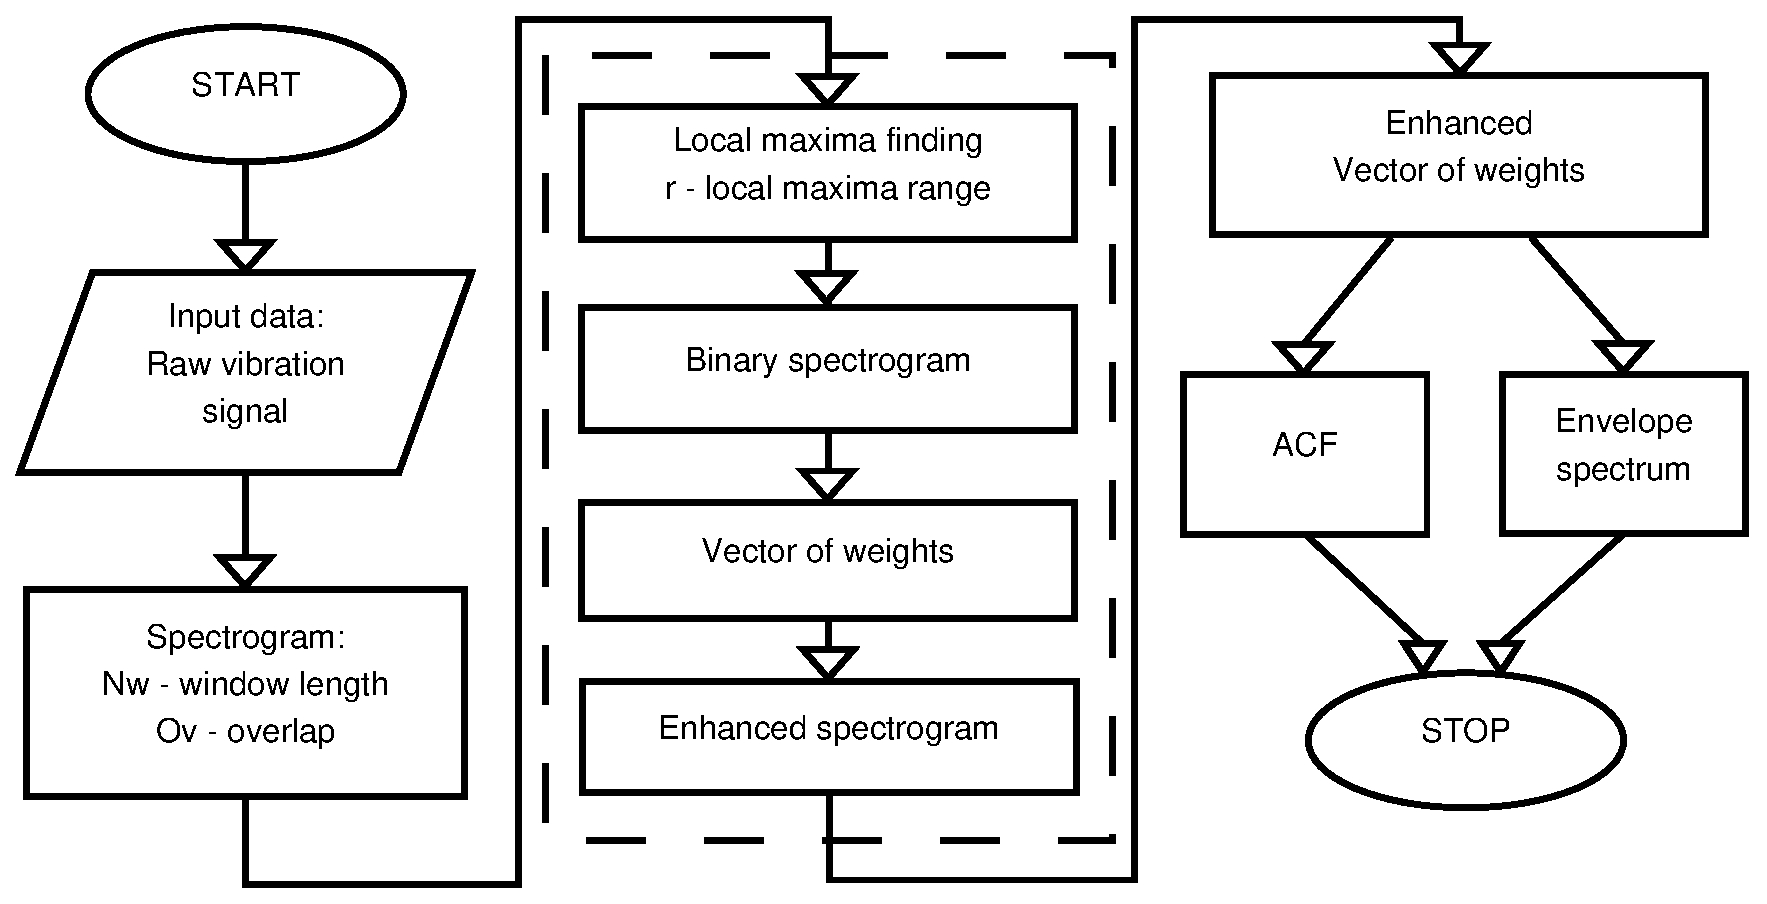
\includegraphics[width=0.7\textwidth]{methodology/tf_enh/fig01diagram}
\caption{Diagram of time-frequency map enhancement procedure.}\label{tf_enh_fig01}
\end{center}
\end{figure}
\FloatBarrier

\section{Selection of informative frequency band}\label{methodology_selection}

In this section we introduce the novel procedure that leads to the local damage detection in rotating machinery. This procedure is based on the time-frequency representation of examined signal. More precisely, in the first step of our analysis we decompose the signal into set of narrowband sub-signals using a time-frequency representation. Here we propose to use the short-time Fourier transform (STFT) that  is defined as follows~\cite{Allen1977235}:
\begin{eqnarray}\label{selection_stft1}
STFT(f,t)=\int_{-\infty}^{\infty}{w(t-\tau)X(\tau)e^{2j\pi f\tau}}\, \mathrm{d} \tau,
\label{selection_stft-cont}\end{eqnarray}
where $w(t-\tau)$ is the shifted window and $X(\tau)$ is the input signal. Discrete version of equation~(\ref{selection_stft1}) for observations $X_1,X_2,...,X_N$, time point $t\in T$ and frequency $f\in \textit{F} $ is defined as follows:
\begin{eqnarray}
STFT(t,f)=\sum_{k=0}^{N-1}X_k w(t-k)e^{2j\pi f k/N}.
\label{selection_stft-discr}\end{eqnarray}
In the second step of our analysis we use several statistics, called selectors, that can be useful as tools for assessment of the sub-signals. Each sub-signal is slice for a given narrow frequency range that arises after mentioned time-frequency decomposition. In this paper we extend the classical approach, where the kurtosis of sub-signals is calculated and propose new selectors based on statistical properties of examined sub-signals. The primary analysis of rotating machinery indicates that sub-signals related to machine in healthy condition are closer to Gaussian than sub-signals related to a damaged one, so some of the proposed statistics are based on the distance between empirical distribution of examined sub-signal and the base distribution, namely the Gaussian one. The selectors mentioned in this paper might be grouped with respect to their statistical properties. In the following subsections we describe the selectors grouped with respect to their statistical properties.
\subsection{Moment-based selectors}
One of the most popular selectors that might be applied to local damage detection of underlying signal is the spectral kurtosis ($SK$),~\cite{Antoni2006308}. The spectral kurtosis  was first introduced as a statistical tool which can indicate not only non-Gaussian components in a signal, but also their locations in the frequency domain. The spectral kurtosis at the frequency band $f$ is defined as follows~\cite{Antoni2006308}:
\begin{eqnarray}\label{selection_spectral_kurtosis}
SK(f)=\#T\frac{\sum_{t\in T}|STFT(t,f)|^4}{(\sum_{t\in T}|STFT(t,f)|^2)^2}-2,
\end{eqnarray}
where $\#T$ denotes the number of elements of the set $T$, i.e. number of time points at which STFT is calculated.\\
Since the spectral kurtosis is based on the fourth-order moment, this group of selectors will be complemented with a statistic which is based on both fourth and third moment, namely the Jarque-Bera statistic. It is strictly related to the Jarque-Bera test, which is a goodness-of-fit test of whether sample data has the skewness and kurtosis matching a normal distribution. This methodology is an extension of the  widely used scheme where only the empirical kurtosis is being investigated. The $JB$ statistic calculated for sub-signal corresponding to frequency band $f$ is defined as:
\begin{eqnarray}
JB(f)=\frac{\#T}{6}\left(S_f^2+\frac{\left(K_f-1\right)^2}{4}\right),
\end{eqnarray}
where $S_f$ and $K_f$ are the empirical skewness and kurtosis, respectively, calculated for given sub-signal corresponding to frequency band $f$.\\
The value of the $JB$ statistic forms a random variable which converges to zero if the underlying distribution has skewness zero and kurtosis 3 (e.g. Gaussian). Any deviation from zero skewness and kurtosis equal to 3 increases the $JB$ statistic.  In this paper the $JB$ statistic is one of the proposed selectors used for local damage detection. If the data come from a normal distribution, the $JB$ statistic asymptotically has a chi-squared distribution with two degrees of freedom, so the statistic can be used to test the hypothesis that the data are derived from a Gaussian distribution. The null hypothesis is a joint hypothesis of the skewness being zero and the excess kurtosis being zero. As the definition of $JB$ shows, any deviation from these values increases the JB statistic.\\
\subsection{ECDF-based selectors}
In this section we describe selectors based on the empirical cumulative distribution function (ECDF). The fundamental statistical property of them is that, for specific distributions, moments of a random variable might be infinite, while cumulative distribution function is always well-defined. Moreover, these two groups are different from the computational point of view - calculating ECDF requires sorting of the sample.\\
The first proposed selector in this group is a Kolmogorov-Smirnov  statistic ($KSS$) that for sub-signal corresponding to the frequency band $f$ is defined as follows~\cite{Corder2009,Justel1997251}:
\begin{eqnarray}\label{selection_K-S}
KSS(f)=sup_x\left|ECDF_f(x)-\Phi_f(x)\right|,
\end{eqnarray}
where $\Phi_f$ is the cumulative distribution function of the Gaussian distribution with parameters estimated from the sub-signal corresponding to the frequency band $f$. Therefore this function is given by:
\begin{eqnarray}\label{selection_FF}\Phi_f(x)=\int^{x}_{-\infty} \! \frac{1}{\sqrt{2\pi\widehat{\sigma_f}^2}}\exp \left( -\frac{\left(x-\widehat{\mu_f}\right)^2}{2\widehat{\sigma_f}^2} \right) \, \mathrm{d} x,\end{eqnarray}
where $\widehat{\mu_f}$ is the empirical mean of the sub-signal $\{|STFT(t,f)|\}_{t\in T}$, and $\widehat{\sigma_f}$ is the empirical standard deviation of  $\{|STFT(t,f)|\}_{t\in T}$. Moreover $ECDF_f(x)$ is the empirical cumulative distribution function calculated for the sub-signal corresponding to the frequency band $f$:
\begin{eqnarray}\label{selection_ECDF}
ECDF_f(x)=\frac{1}{\#T}\sum_{t\in T}\mathbf{1}\left\{ |STFT(t_k,f)|\leq x\right\}
\end{eqnarray}
In the above definition $\mathbf{1}\{A\}$ denotes the indicator of the set A.\\
\begin{figure}[!ht]
\begin{center}
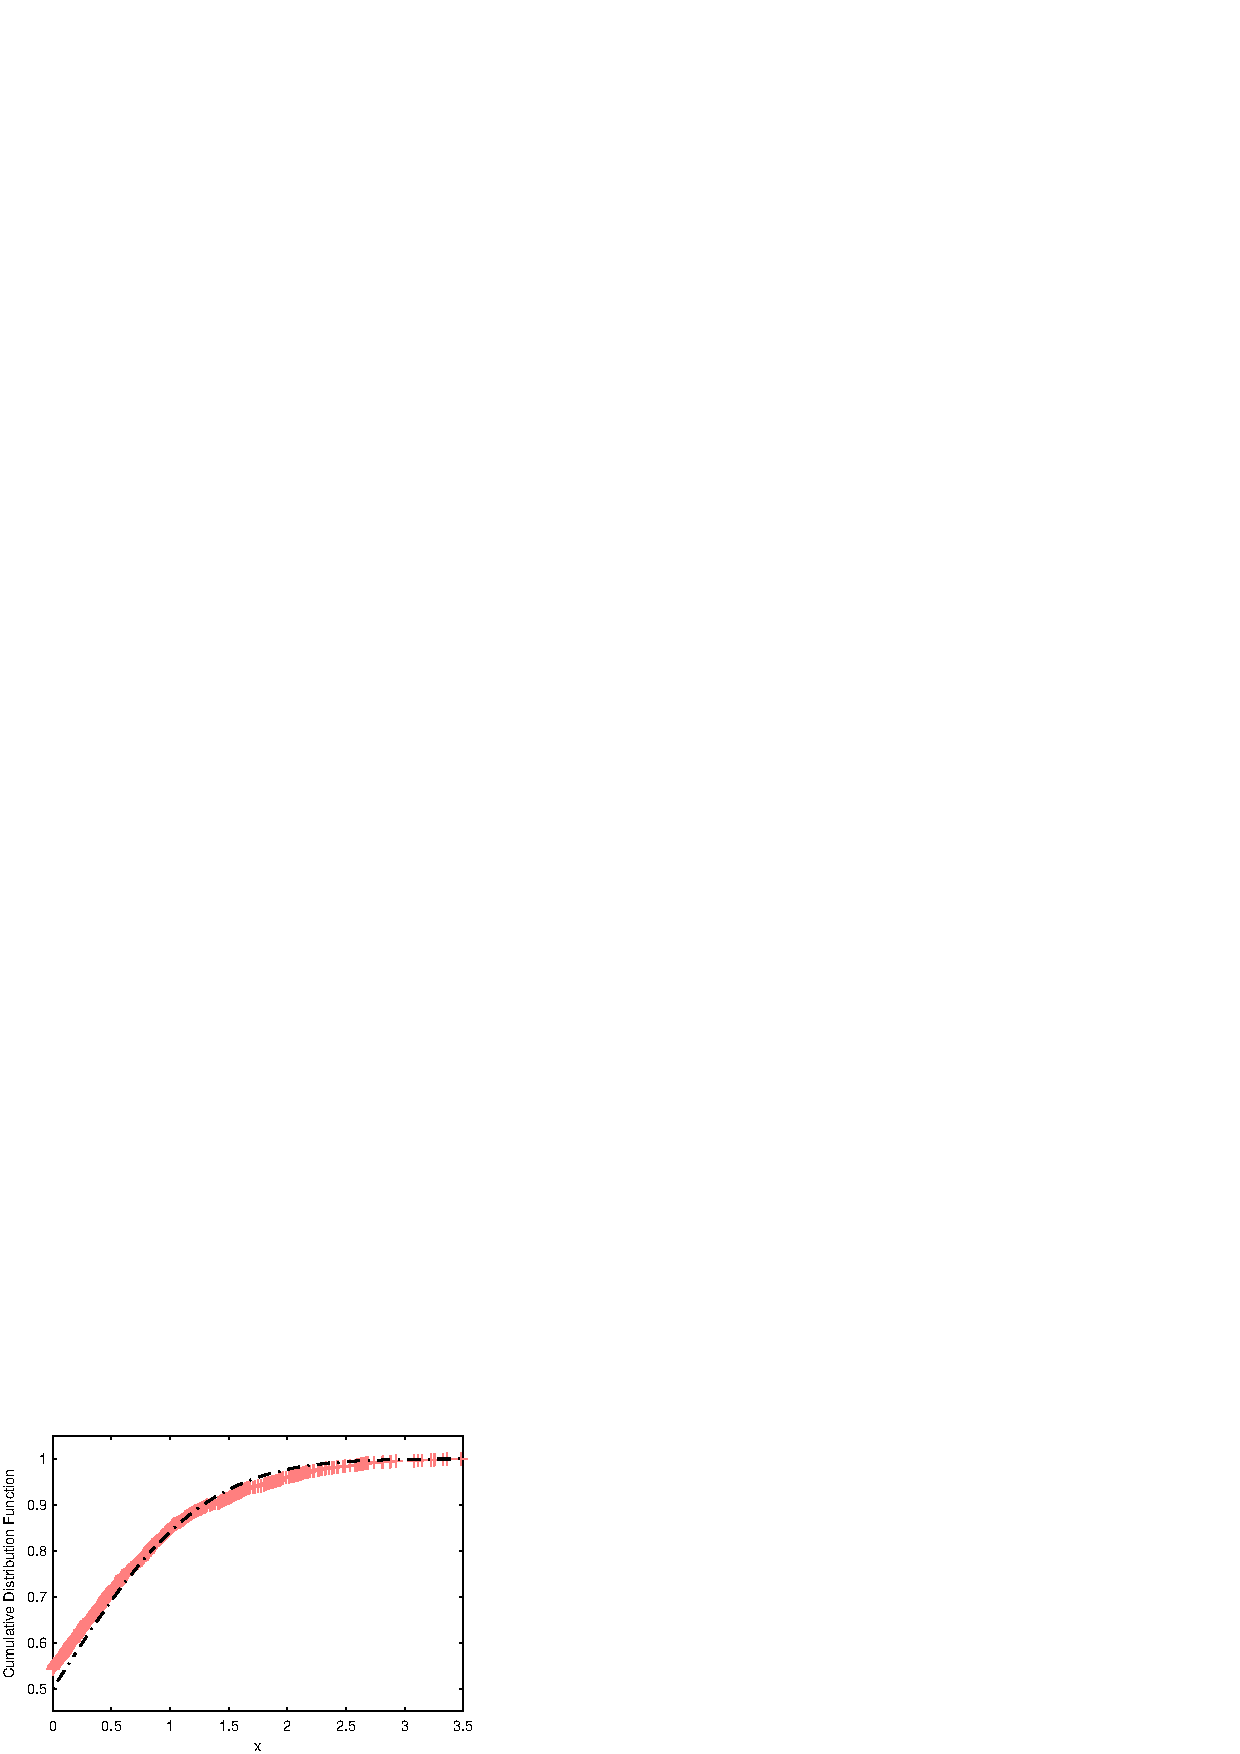
\includegraphics[width=0.4\textwidth]{methodology/selection/fig01aecdf_g}
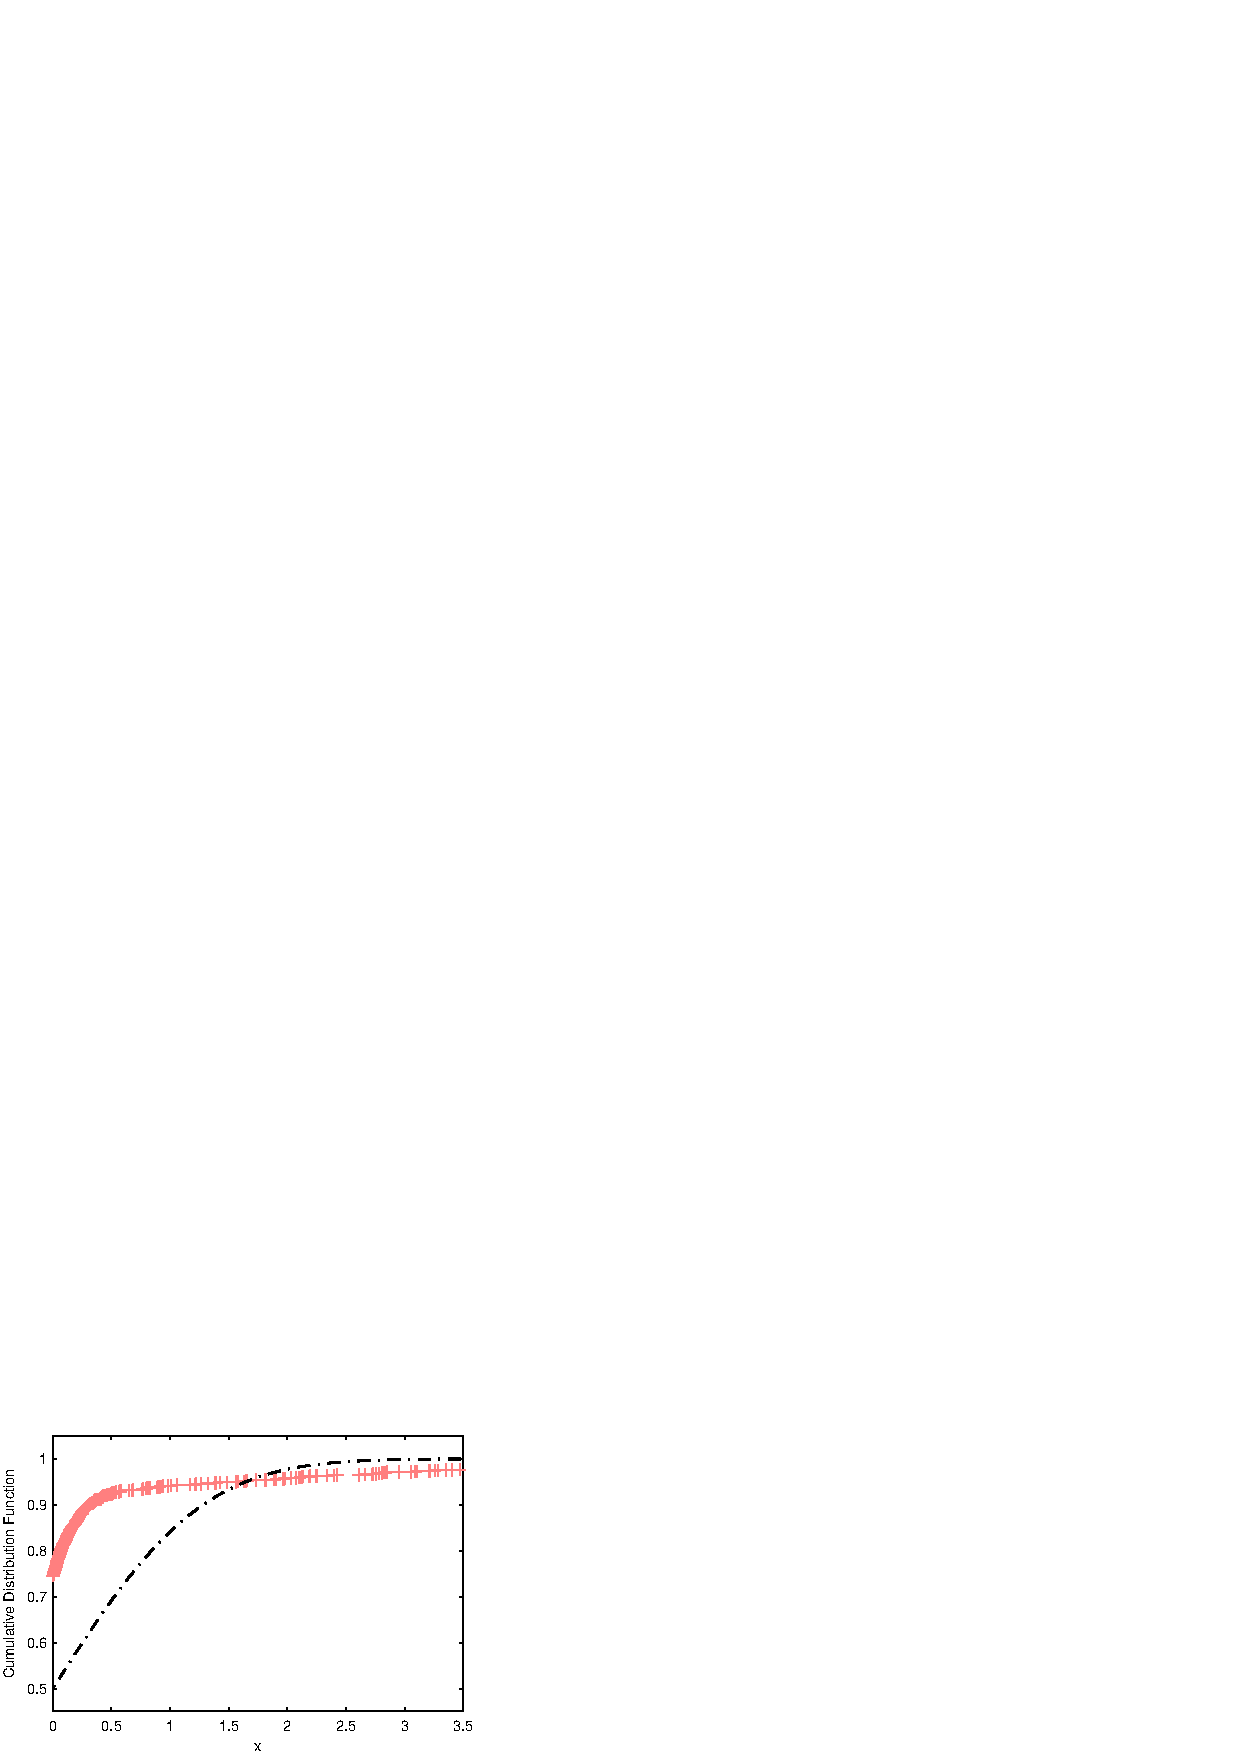
\includegraphics[width=0.4\textwidth]{methodology/selection/fig01becdf_b}
\caption{The empirical and theoretical (Gaussian) cumulative distribution functions for exemplary sub-signals from machine in good condition (left panel) and damaged one (right panel). The black dashed line represents the reference cumulative distribution function of Gaussian distribution.}\label{selection_fig1}
\end{center}
\end{figure}
The idea of using the Kolmogorov-Smirnov statistic for spikiness detection is illustrated in Fig.~\ref{selection_fig1}, where we present the empirical and theoretical cumulative distribution functions for real data set analyzed in Sec.~\ref{selection_bearing}. In the left panel of Fig.~\ref{selection_fig1} we show the cumulative distribution functions (empirical and theoretical - Gaussian) for sub-signal corresponding to the frequency $f=2325$~Hz for machine in good condition while in the right panel for the damaged one. One can observe in the left panel the analyzed functions are closer than in the right panel, therefore the $KSS$ for this frequency band has lower value for the sub-signal from machine in good condition.\\ In~\cite{Stephens1979591,Burnecki2011293} one can find more properties of the $KSS$ statistic and statistical test based on it. We only mention here the $KSS$ statistic tends to zero (almost surely) when number of elements in set $T$ tends to infinity. Moreover the distribution of $KSS$ statistic defined in (\ref{selection_K-S}) is normal. The first fact is a result of Glivenko-Cantelli theorem~\cite{Tucker1959828} while the second it is so called the distribution-free property.\\
The next statistic that might be a useful tool for informative band selection is an extension of the mentioned Kolmogorov-Smirnov. Similar to $KSS$, it is based on the distance between theoretical and empirical cumulative distribution functions for underlying sub-signal. The selector, called Anderson-Darling statistic, belongs to the Cramer-von Mises family of statistics which incorporate the idea of quadratic norm. The Cramer-von Mises statistic for frequency band $f$ is defined by~\cite{Burnecki2011293}
\begin{eqnarray}
Q(f)=\#T\int^{\infty}_{-\infty} \! \left(ECDF_{f}\left(x \right) - \Phi_f\left(x\right)\right)^2 \phi \left(x\right) \, \mathrm{d} x
\end{eqnarray}
where $\phi \left(x\right)$ is a suitable function which puts weights to the squared difference $\left(ECDF_{f}\left(x \right) - \Phi_f\left(x\right)\right)^2$. Moreover functions $ECDF_f(x)$ and $\Phi_f(x)$ are defined in (\ref{selection_FF}) and (\ref{selection_ECDF}), respectively. When $\phi(x)=1$, $Q(f)$ is called the Cramer-von Mises statistic. In this case we denote it as $CVM$. If $\phi\left(x\right)=\left[ \Phi_f\left(x\right) \left( 1-\Phi_f\left(x\right) \right) \right]^{-1}$, the above definition yields the Anderson-Darling statistic.  In the further analysis it is denoted as $AD$. Similarly to the Kolmogorov-Smirnov statistic there exist statistical tests that allow to test the proper distribution of examined data by using the $CVM$ and $AD$ statistics. More details can be found in~\cite{Anderson1952193,Anderson1954765,Burnecki2012}. The Cramer-von Mises test has better properties than the Kolmogorov-Smirnov test, but it is relatively insensitive to "tails" of the distribution. In order to eliminate this disadvantage the Anderson-Darling test was introduced. The Anderson--Darling test is a statistical test of whether a given sample of data is drawn from a given probability distribution. In our case the base distribution is normal. The test is one of the most powerful statistical tools for detecting deviations from normality.\\
\subsection{Quantile-quantile plot-based selectors}
Except of statistical tests with explicit hypothesis, there are some visual tests to compare two distributions, e.g. the theoretical distribution and the empirical one. One of the most famous examples is the quantile-quantile plot (QQplot),~\cite{Cleveland1994}. Plot of the theoretical distribution quantiles versus the underlying ones might be useful to recognize goodness-of-fit. Straight line on the QQplot means that compared distributions have the same shape. Straight line with equal scales on the axes means equal distributions. If there is no straight line, then one can compare, for example, tail heaviness of both distributions. In most of numerical packages (MATLAB, R) there is an additional straight line plotted to make analysis easier. This line connects two points: first and third quartiles of both distributions. To make this test numerical, we propose to measure the horizontal distance between the QQplot markers and the additional straight line. One can note that statistics contained in this group require sorting, similar to the previous group. Nevertheless, the lack of explicit hypothesis of gaussianity test based on the QQplot tends us to classify them into an individual group.\\
\begin{figure}[!ht]
\begin{center}
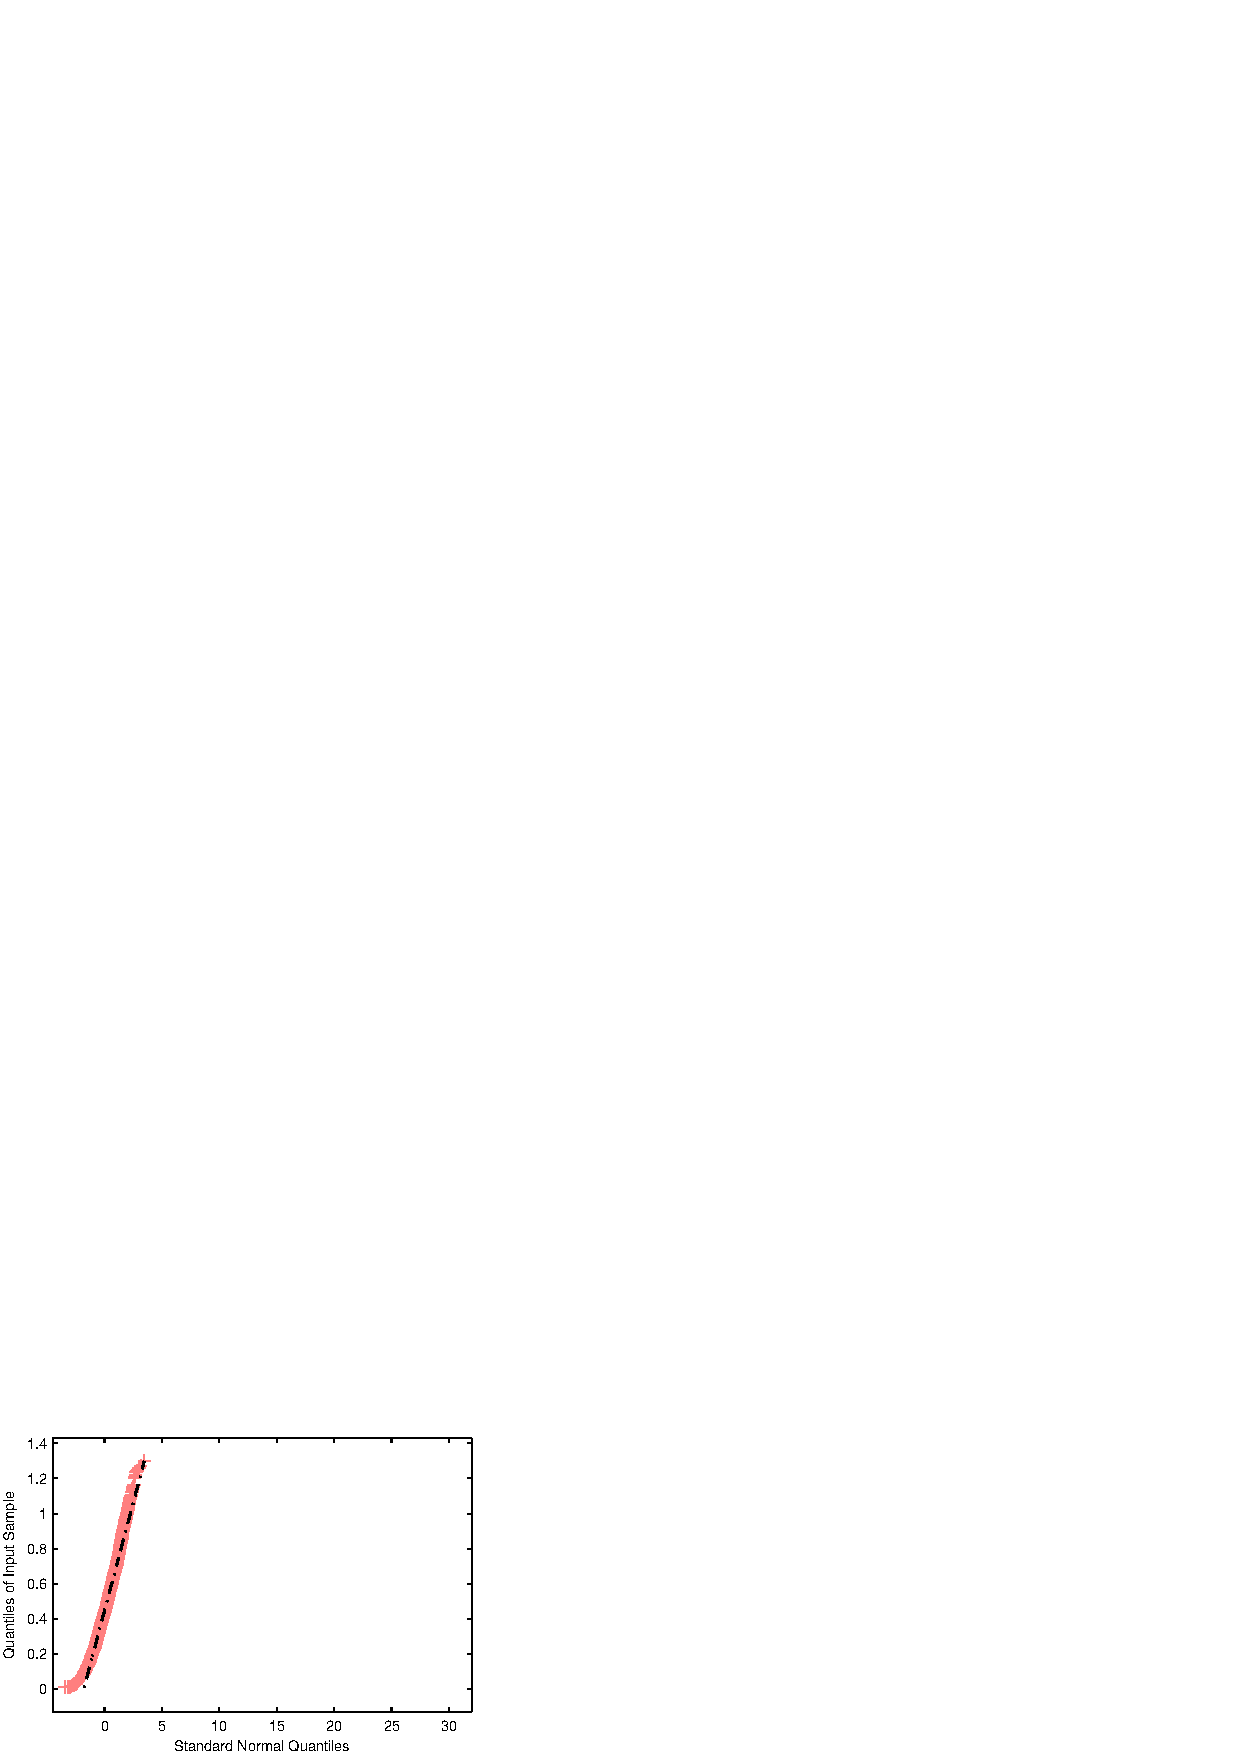
\includegraphics[width=0.4\textwidth]{methodology/selection/fig02aqqplot_g}
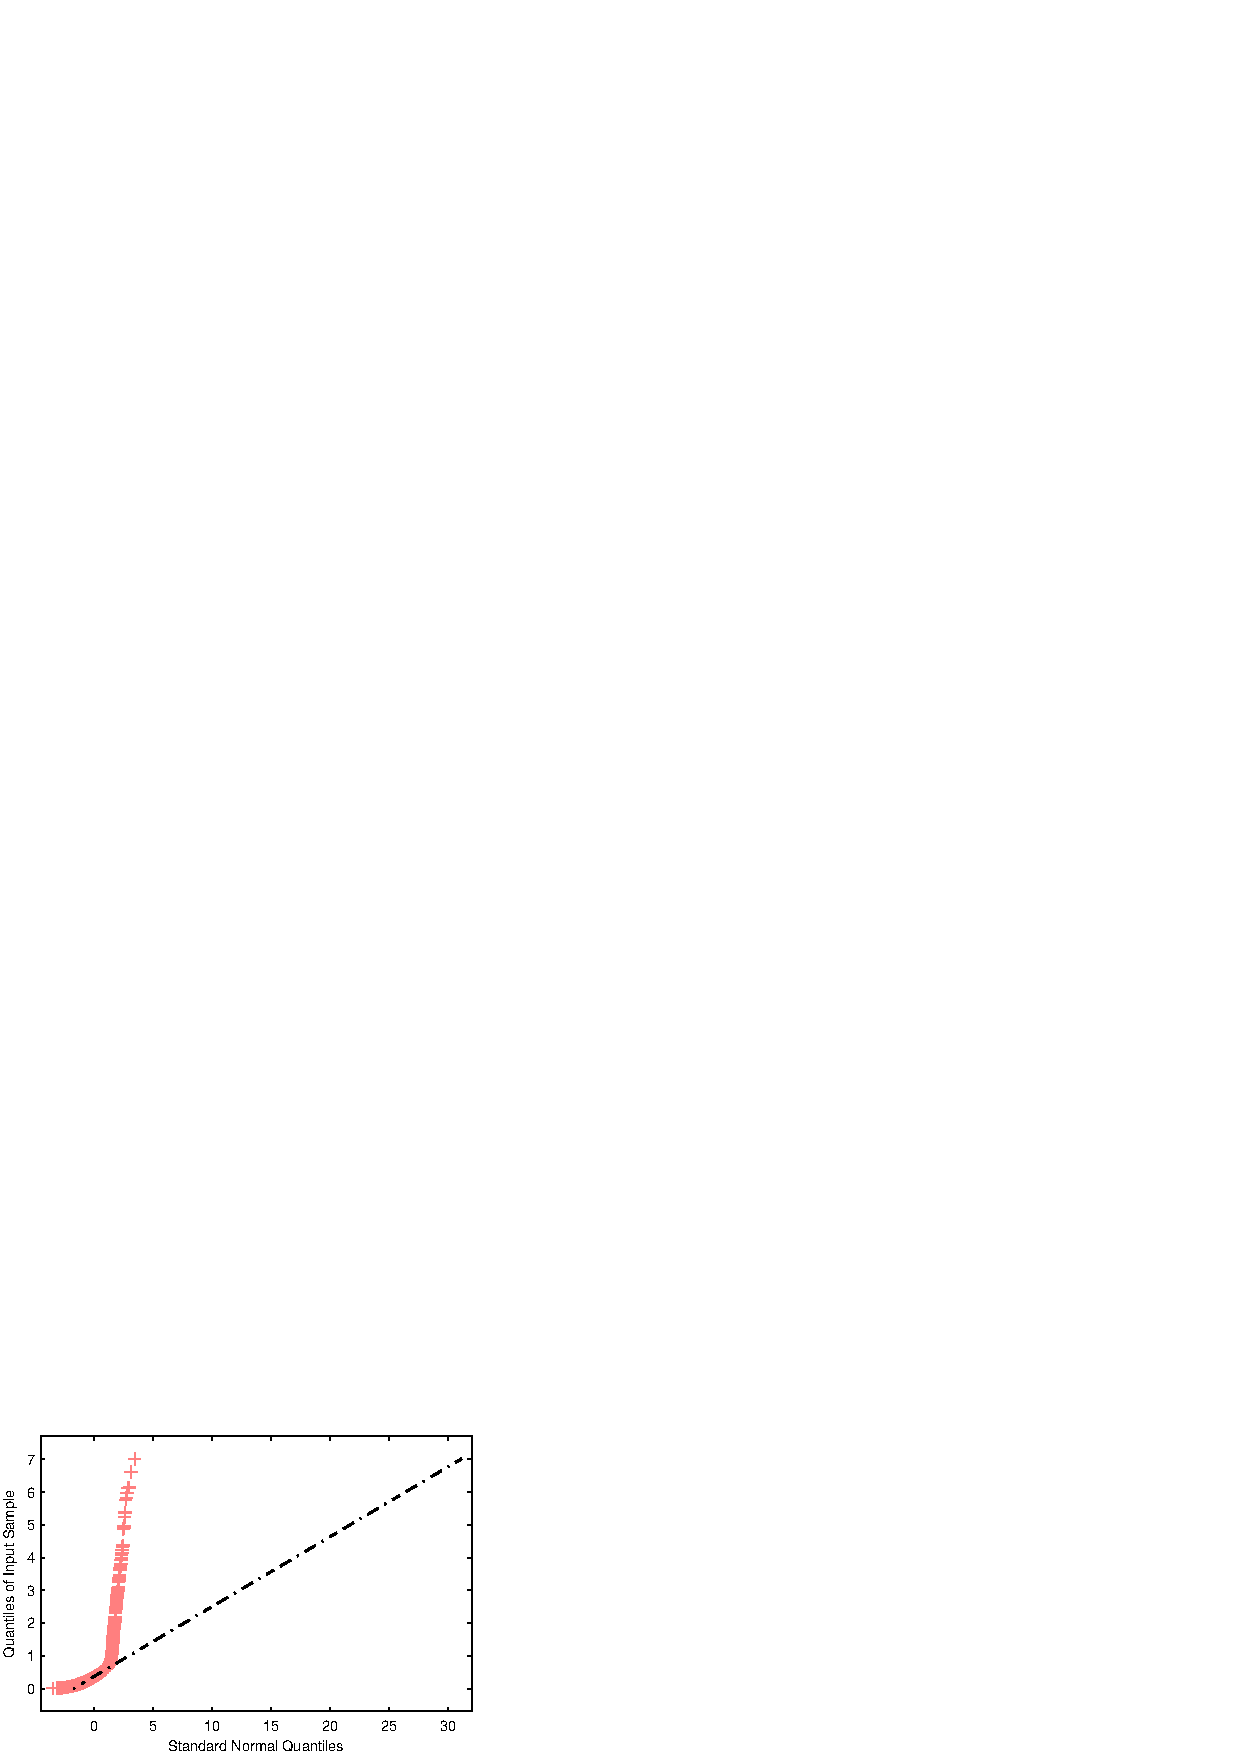
\includegraphics[width=0.4\textwidth]{methodology/selection/fig02bqqplot_b}
\caption{QQplot of the healthy (left panel) and unhealthy (right panel) sub-signal compared to the normal distribution. The black dashed line represents the reference quantile line for Gaussian distribution. Note that only horizontal distance between markers and line is quantified by $H_{aver}$ and $H_{max}$.}\label{selection_fig2}
\end{center}
\end{figure}
For this test, we propose to compute mean and maximum of those distances. The formula for the maximum distance between the Gaussian distribution and the sub-signal corresponding to the frequency band $f$ is as follows:
\begin{eqnarray}
H_{max}(f)=\max_{1\leq k \leq \#T}{ \left| \Phi^{-1}_f\left( \frac{2k-1}{2\#T} \right) - a S(k,f)-b \right| },
\end{eqnarray}
where $\Phi_f^{-1}$ is the inverse of $\Phi_f$ defined in (\ref{selection_FF}) for $\mu=0$ and $\sigma=1$, $S(k,f)$ is the $k$-th value of ascending sorted sub-signal $\{|STFT(t,f)|\}_{t\in T}$, $a=\dfrac{\Phi^{-1}(0.75)-\Phi^{-1}(0.25)}{q_{f}(0.75)-q_{f}(0.25)}$, $b=\Phi^{-1}(0.75)-aq_{f}(0.75)$ and $q_{f}(p)$ is a $p$-th order quantile of a sub-signal $\{|STFT(t,f)|\}_{t\in T}$. The formula for the average distance is analogous with the $\max$ function substituted by the arithmetic mean. We denote the corresponding statistic as $H_{aver}$. The exemplary QQplots  for real data examined in Sec.~\ref{selection_bearing} of a healthy signal (for a given frequency bin) is presented in Fig.~\ref{selection_fig2} (left panel) while for the sub-signal with defect - in the right panel of Fig.~\ref{selection_fig2}. We observe the healthy signal is closer to Gaussian distribution than the unhealthy one. Both average and maximum horizontal distances between straight line and markers are significantly larger in the right panel.
\subsection{Local maxima method-based selector}
The last procedure that allows for construction of a selector for local damage detection is based on the local maxima method~\cite{Obuchowski2014325,Obuchowski2014389}. For each frequency band (i.e. each sub-signal) we check the local maximum occurrence. We assume that local maximum occurs at a given time point when the modulus of STFT value therein is higher than the other values in its neighborhood of a length not less than a certain value - $r$. Then, for each frequency band we create a new binary vector which is a transformation of the original data into zero-one series. More precisely, we put 1 at a time point when the local maximum occurs and 0 otherwise. Let us point that the binary values obtained in this way minimize influence of insignificant signals for local damage detection as well as maximize influence of characteristic signals for locally damaged machinery. In our methodology for each time point we use the vector of weights (VoW), which is a vector of averaged maxima occurrence, i.e. VoW at point $t$ is defined as follows:
\begin{eqnarray}
W(t)=\frac{1}{\#\textit{F}}\sum_{f\in\textit{ F}}M(t,f),
\end{eqnarray}
where $M(t,f)$  represents binary valued vector of the local maxima occurrence at the time point  $t$ and frequency $f$. After multiplying each previously computed binary value by the value of VoW at the corresponding time point we obtain an enhanced spectrogram. Therefore the enhanced spectrogram at point $(t,f)$ is defined as follows:
\begin{eqnarray}
ENH(t,f)=W(t)M(t,f).
\end{eqnarray}
More details of the procedure for the enhanced spectrogram construction for different applications one can find in~\cite{Obuchowski2014325,Obuchowski2014389}. The selector based on the local maxima method for frequency band $f$ is constructed as follows:
\begin{eqnarray}
LM(f)=\frac{1}{\#T}\sum_{t\in T}ENH(t,f).
\end{eqnarray}
\FloatBarrier

\section{Linear filter design based on selectors}\label{methodology_filtering}

In this section we present the whole methodology which leads to the raw vibration signal enhancement. It is composed of 4 steps (Fig.~\ref{filtering_fig1}):
\begin{itemize}
\item{decomposition of the signal into two-dimensional time-frequency plane,}
\item{selector values calculations for informative band selection,}
\item{estimation of thresholds for individual frequency bins,}
\item{filtering of raw vibration signal and envelope analysis.}
\end{itemize}
At first, the signal is decomposed into a time-frequency map (STFT), which is an estimate of energy fluctuation at particular frequency bins in time. Specifically, we process sub-signals, i.e. time series associated with a particular frequency bin. Each sub-signal is examined how far from Gaussian is its empirical distribution. In order to do this, we examine values of several selectors calculated for every sub-signal. The selectors are based on statistical moments, empirical quantiles and cumulative distribution function. As one of the selectors we use the spectral kurtosis.\\
For a given selector, we obtain a set of weights for the whole signal's spectrum. The weights are used to establish a linear filter similar to the Wiener filter based on the SK~\cite{Combet2009652}. Filtering incorporates the discrete Fourier transform (DFT) and its inverse. In order to enhance filter's amplitude response we propose to cut-off the selector values using individual thresholds for each frequency bin. The thresholds are calculated upon reference signals, whose amplitude spectra are similar to the amplitude spectrum of the raw vibration signal. The reference signals are simulated using the Monte Carlo method and a procedure called inverse pre-whitening.\\
After the thresholds are calculated and selector values are enhanced, we propose to filter the signal in frequency domain. Then, the signal's envelope spectrum is analyzed.
\begin{figure}[!t]
\centering
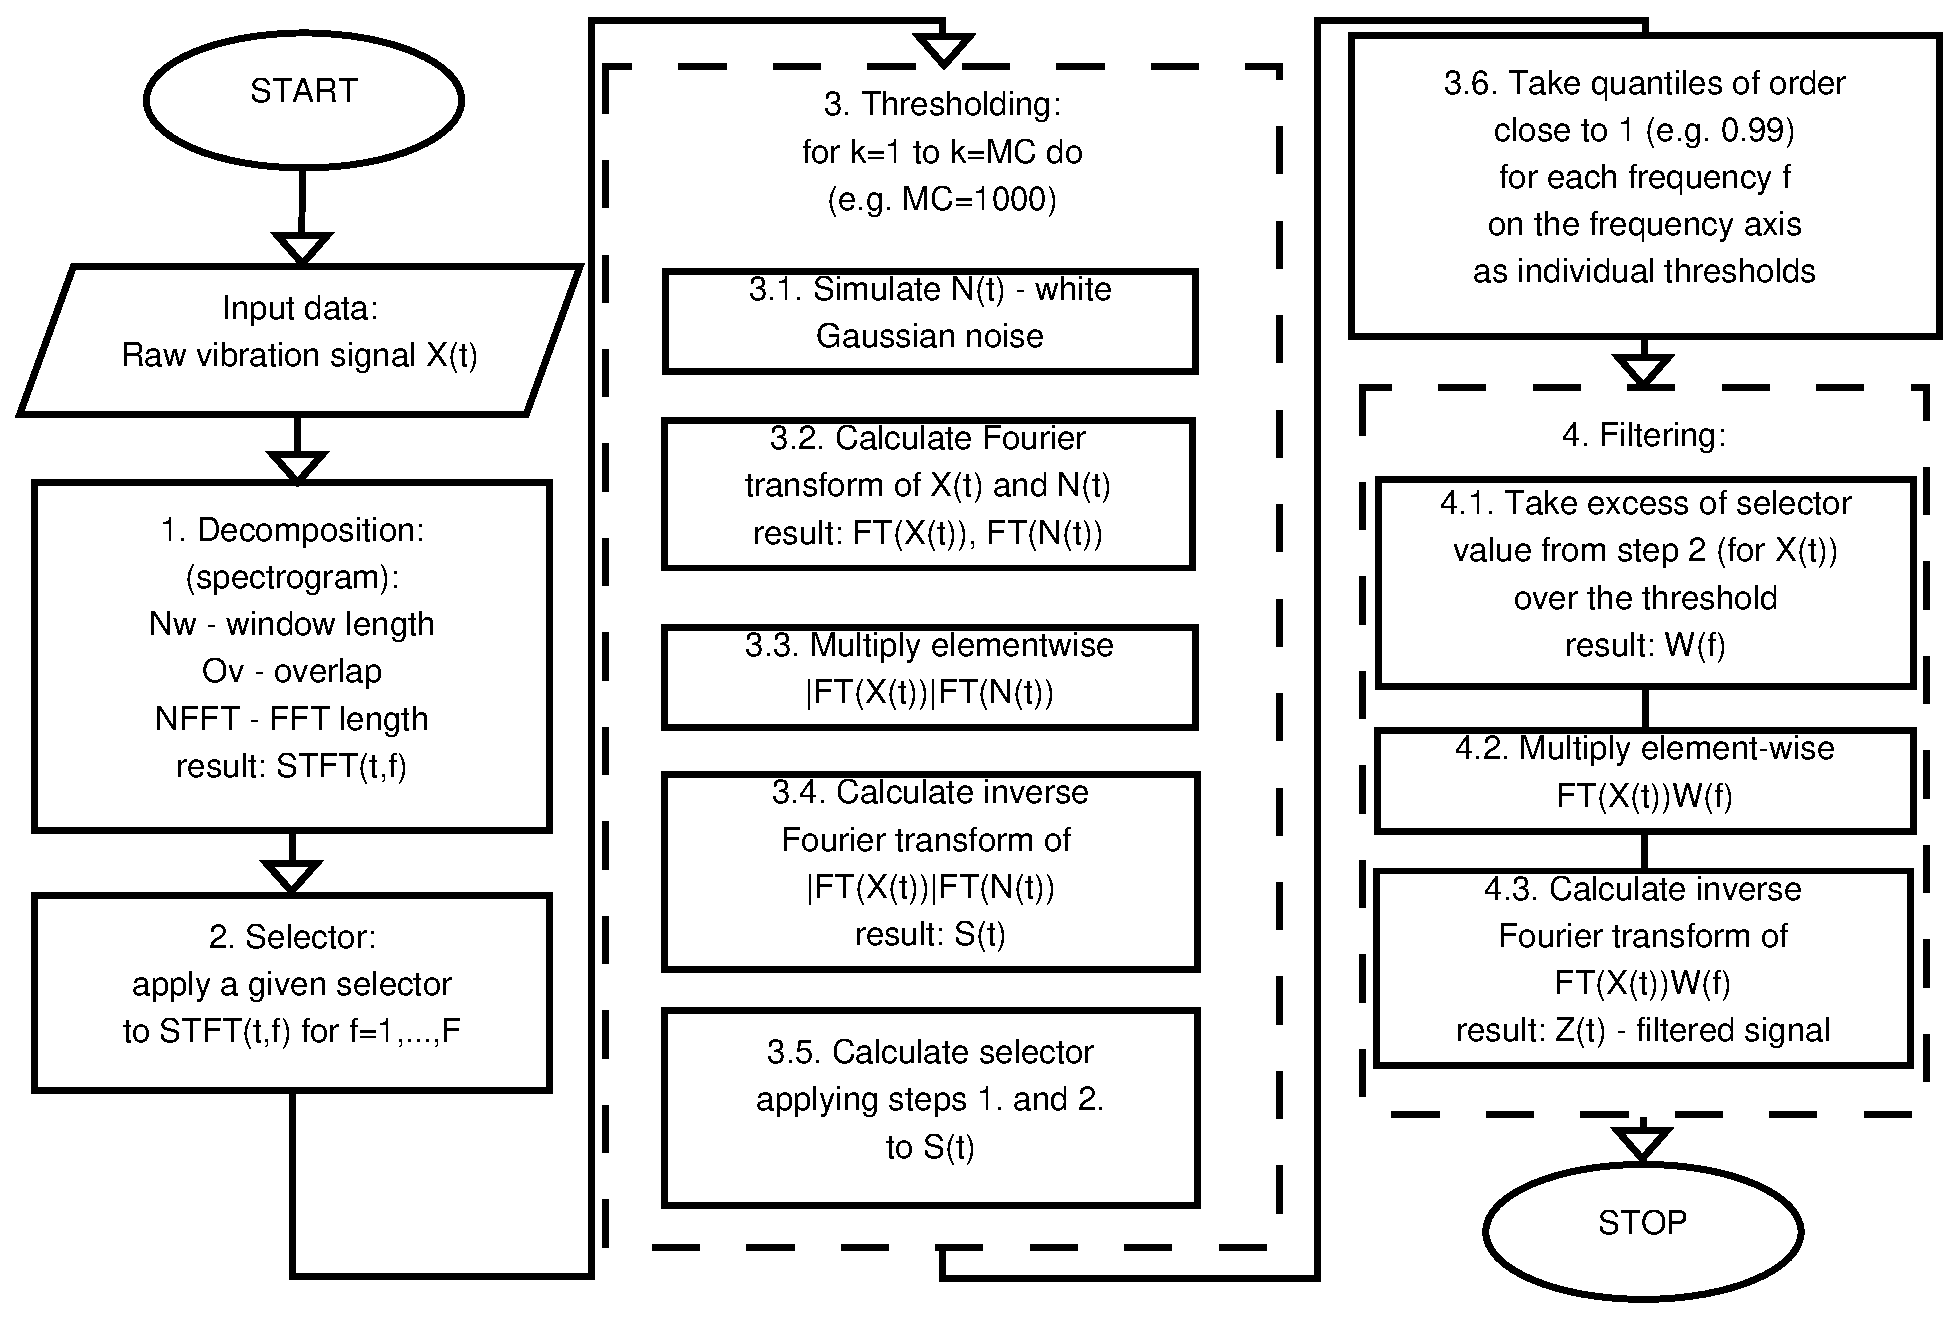
\includegraphics[width=1\textwidth]{methodology/filtering/Diagram2}
\caption{Block diagram of the filtering procedure.}
\label{filtering_fig1}
\end{figure}
\subsection{Decomposition}\label{filtering_decomposition}
Decomposition is based on analysis of the discrete short-time Fourier transform (STFT) which for $x_1,x_2,...,x_N$, time point $t= \left\{1,\ldots,T\right\}$ and frequency $f= \left\{1,\ldots,F\right\}$ is defined as follows~\cite{Allen1977235}:
\begin{eqnarray}
STFT(t,f)=\sum_{k=0}^{N-1}x_k w(t-k)e^{-2j\pi f k/N},
\label{filtering_stft-discr}\end{eqnarray}
where $w(t-k)$ is the shifted window and $x_k$ is the input signal. The window (length and shape) affects the final result in the similar manner as in the spectral kurtosis case. In this paper we present results obtained by using 80\% overlapping.
\subsection{Selectors}\label{filtering_selectors}
In this section we recall four selectors~\cite{Obuchowski2014138,Obuchowski2013441}, each of them could be a base for a linear filter. For comparison, one of the selectors is the classical spectral kurtosis. Recall, that the SK is based on the fourth-order statistic. The spectral kurtosis at the frequency bin $f$ is defined as follows~\cite{Antoni2006308}:
\begin{eqnarray}
SK(f)=T\frac{\sum_{t=1}^{T}|STFT(t,f)|^4}{(\sum_{t=1}^{T}|STFT(t,f)|^2)^2}.\label{filtering_spectral_kurtosis}
\end{eqnarray}
Besides the ability of a pulse train detection, the $SK$ is also very sensitive to a single non-informative impulse that might occur, for instance, during the signal acquisition. In the classical definition, the sum in~(\ref{filtering_spectral_kurtosis}) is reduced by 2 which stands for a cut-off threshold, i.e. only the values of $SK(f)$ larger than 2 are significant. In our approach such subtraction is not necessary - the thresholding procedure quantifies the significance of each selector's value and takes into account only the excess over the threshold.\\
The second selector is the Jarque-Bera statistic~\cite{Jarque1980255,Burnecki2012}. It is based on both kurtosis and skewness. The $JB$ at $f=1,\ldots,F$ is defined as follows:
\begin{eqnarray}
JB(f)=\frac{T}{6}\left(S(f)^2+\frac{\left(K(f)-3\right)^2}{4}\right),
\end{eqnarray}
where $S(f)$ and $K(f)$ are the empirical skewness and kurtosis, respectively, calculated for a given sub-signal, corresponding to the frequency bin $f$. $JB$ exploits not only the fourth, but the third moment as well, in order to examine gaussianity of the random sample. Thus, it might indicate asymmetry of distribution, which occurs in specific types of damage in rotating machines~\cite{Ovacikli2013462}. The higher value of $JB$, the more the distribution of the sample differs from the Gaussian distribution.\\
The next selector is based on a quantile-quantile plot (QQplot). Vertical and horizontal axes of the QQplot are here related to quantiles of empirical sub-signal's distribution and the standard Gaussian distribution, respectively. The selector quantifies the average distance between markers of QQplot and a reference line defined by first and third quartiles of both distributions~\cite{Obuchowski2013441}. The selector $H_{aver}$ at $f=1,\ldots,F$ is defined as~\cite{Obuchowski2014138}:
\begin{eqnarray}
H_{aver}(f)=\frac{1}{T}\sum_{k=1}^{k=T}{ \left| \widetilde{\Phi}^{-1}\left(\frac{2k-1}{2T} \right) - a S(k,f)-b \right| },
\end{eqnarray}
where $\widetilde{\Phi}^{-1}(\cdot)$ is the inverse of cumulative distribution function of the standard Gaussian distribution, i.e. $$\widetilde{\Phi}(x)=\int^{x}_{-\infty} \! \frac{1}{\sqrt{2\pi}}\exp \left( -\frac{x^2}{2} \right) \, \mathrm{d} x,$$ $S(k,f)$ is the $k$-th value of ascending sorted sub-signal $\{|STFT(t,f)|\}_{t=1,\ldots,T}$, $a=\dfrac{\widetilde{\Phi}^{-1}(0.75)-\widetilde{\Phi}^{-1}(0.25)}{q(f,0.75)-q(f,0.25)}$, $b=\widetilde{\Phi}^{-1}(0.75)-aq(f,0.75)$ and $q(f,p)$ is a $p$-th order quantile of a sub-signal $\{|STFT(t,f)|\}_{t=1,\ldots,T}$. In~\cite{Obuchowski2013441} it is shown that this selector distinguishes healthy from faulty bearing's signal as good as SK does, but $H_{aver}$ defines a different order on the set of sub-signals than $SK$ does. Recall that $H_{aver}$ is scale-invariant, since the distance is measured on the axis corresponding to standard normal distribution. Due to the design of $H_{aver}$, one can notice its robustness to single outlying values. One can consider two signals of different lengths, the same statistical distribution and both of them contain a single outlier of similar level. Then $H_{aver}$ is lower for the longer signal, since the appropriate quartiles and $S(k,f)$'s are similar and the denominator, namely $T$, distinguishes these signals.\\
The next selector incorporates the idea of quantifying the distance between the empirical cumulative distribution function (empirical CDF) of the sub-signal and the CDF of the fitted Gaussian distribution. Specifically, it is a Kolmogorov-Smirnov statistic which is defined as follows~\cite{Obuchowski2014138,cordernonparametric,Justel1997251}:
\begin{equation}\label{filtering_K-S}
KSS(f)=sup_x\left|ECDF(f,x)-\Phi(f,x)\right|,
\end{equation}
where $\Phi(f,\cdot)$ is the cumulative distribution function of the Gaussian distribution with mean and variance estimated from the sub-signal corresponding to the frequency bin $f$. Therefore this function is given by:
\begin{eqnarray}\label{filtering_FF}
\Phi(f,x)=\int^{x}_{-\infty} \! \frac{1}{\sqrt{2\pi\widehat{\sigma}(f)^2}}\exp \left( -\frac{\left(x-\widehat{\mu}(f)\right)^2}{2\widehat{\sigma}(f)^2} \right) \, \mathrm{d} x,
\end{eqnarray}
where $\widehat{\mu}(f)$ is the empirical mean of the sub-signal $\{|STFT(t,f)|\}_{t=1,\ldots,T}$, and $\widehat{\sigma}(f)$ is the empirical standard deviation of $\{|STFT(t,f)|\}_{t=1,\ldots,T}$. Moreover, $ECDF(f,x)$ is the empirical cumulative distribution function calculated for the sub-signal corresponding to the frequency bin $f$:
\begin{eqnarray}\label{filtering_ECDF}
ECDF(f,x)=\frac{1}{T}\sum_{t=1}^{T}\mathbf{1}\left\{ |STFT(t,f)|\leq x\right\}.
\end{eqnarray}
In the above definition $\mathbf{1}\{a\leq x\}$ denotes the indicator function, i.e. $\mathbf{1}\{a\leq x\}=1$ if $a\leq x$ and 0 otherwise. This selector is also scale-invariant. Moreover, in opposite to the previous selectors, $KSS$ is bounded since values of both cumulative distribution functions (i.e. $ECDF$ and $\Phi$) are between 0 and 1.\\
The values of a particular selector for the entire spectrum constitute a ground for the amplitude response of the filter. The following sections provide a complete description how to obtain the final filter that might be used to obtain the informative part of the vibration signal.
\subsection{Thresholding}\label{filtering_thresholding}
Once the amplitude response of the filter is calculated, it has to be enhanced in order to take into account the significant values of the selector only. We propose to design significance thresholds for each frequency bin individually.
\begin{figure}[!ht]
\begin{center}
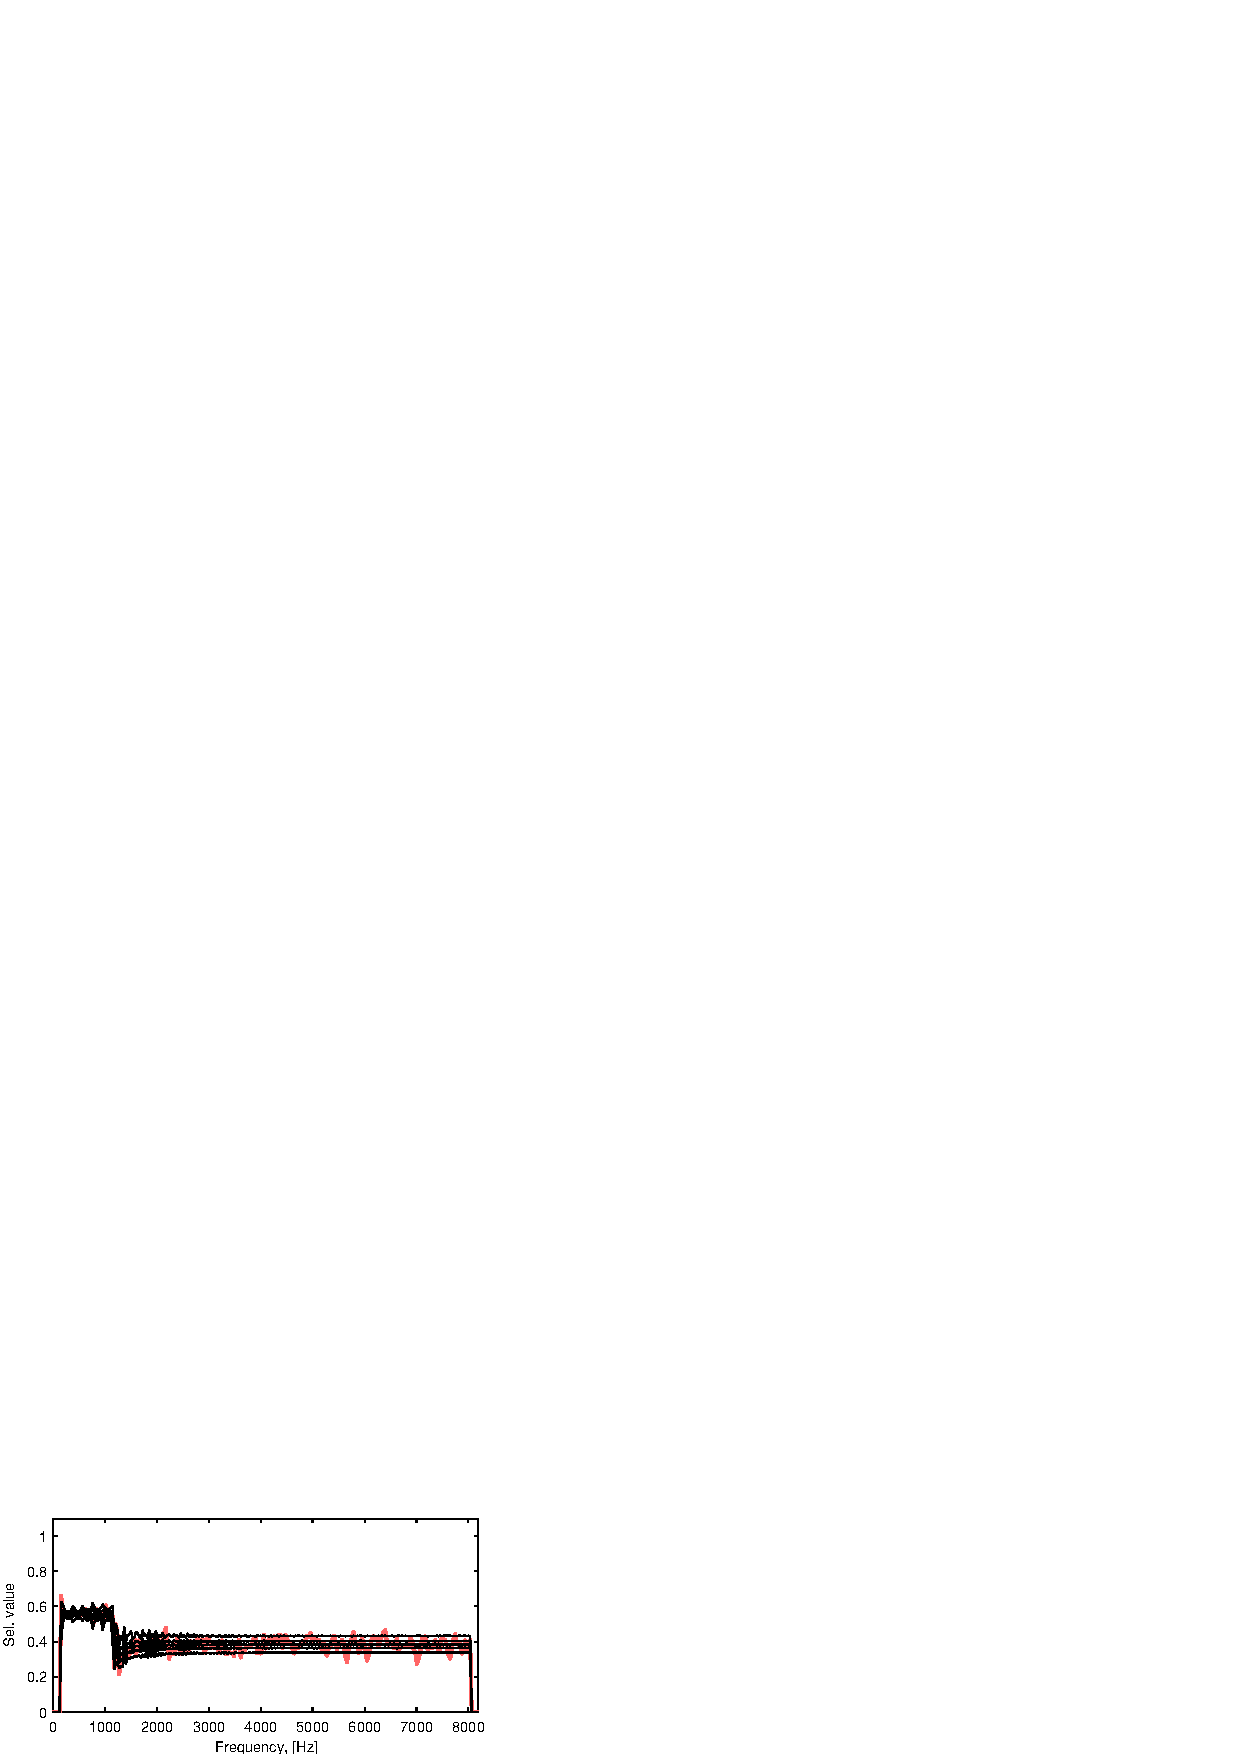
\includegraphics[width=0.49\textwidth]{methodology/filtering/sin_const-quantile_lines_g}
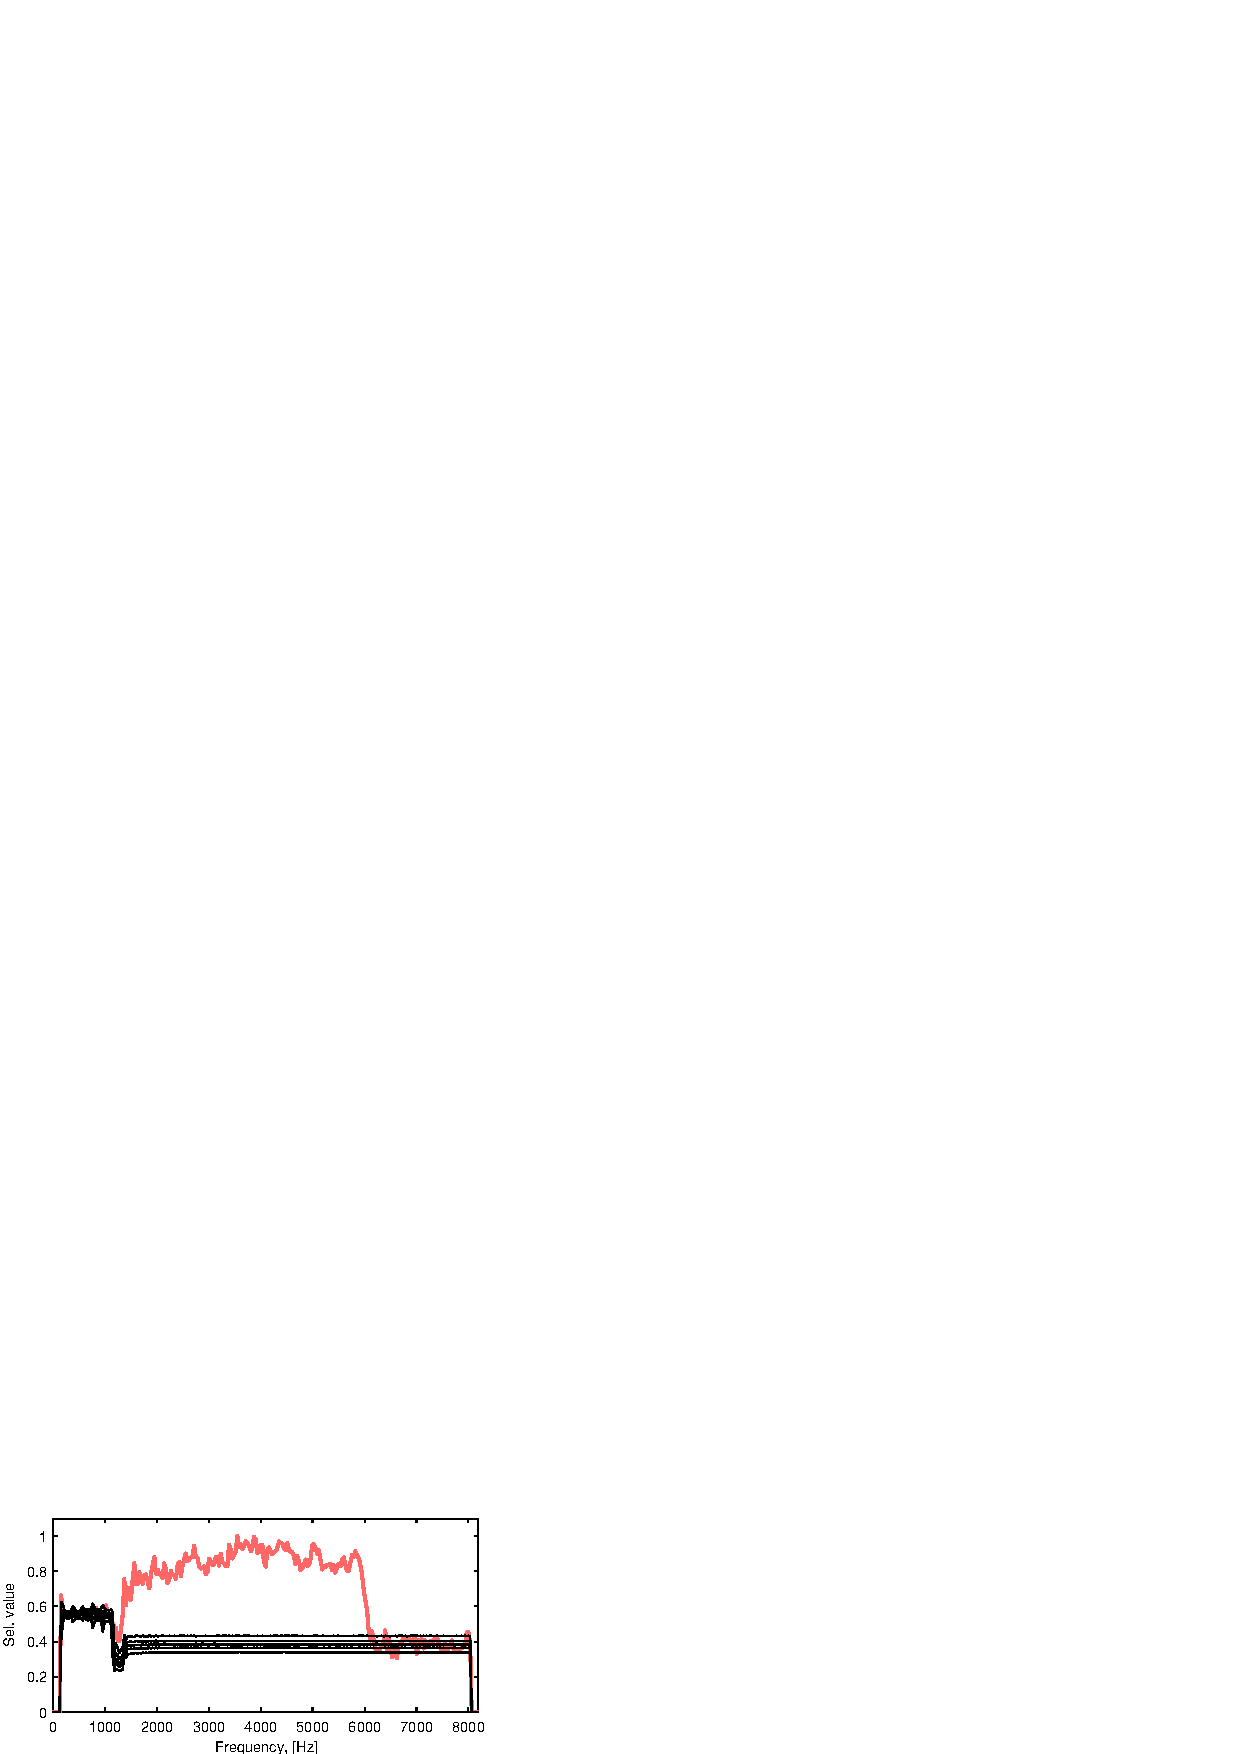
\includegraphics[width=0.49\textwidth]{methodology/filtering/sin_const-quantile_lines_b}
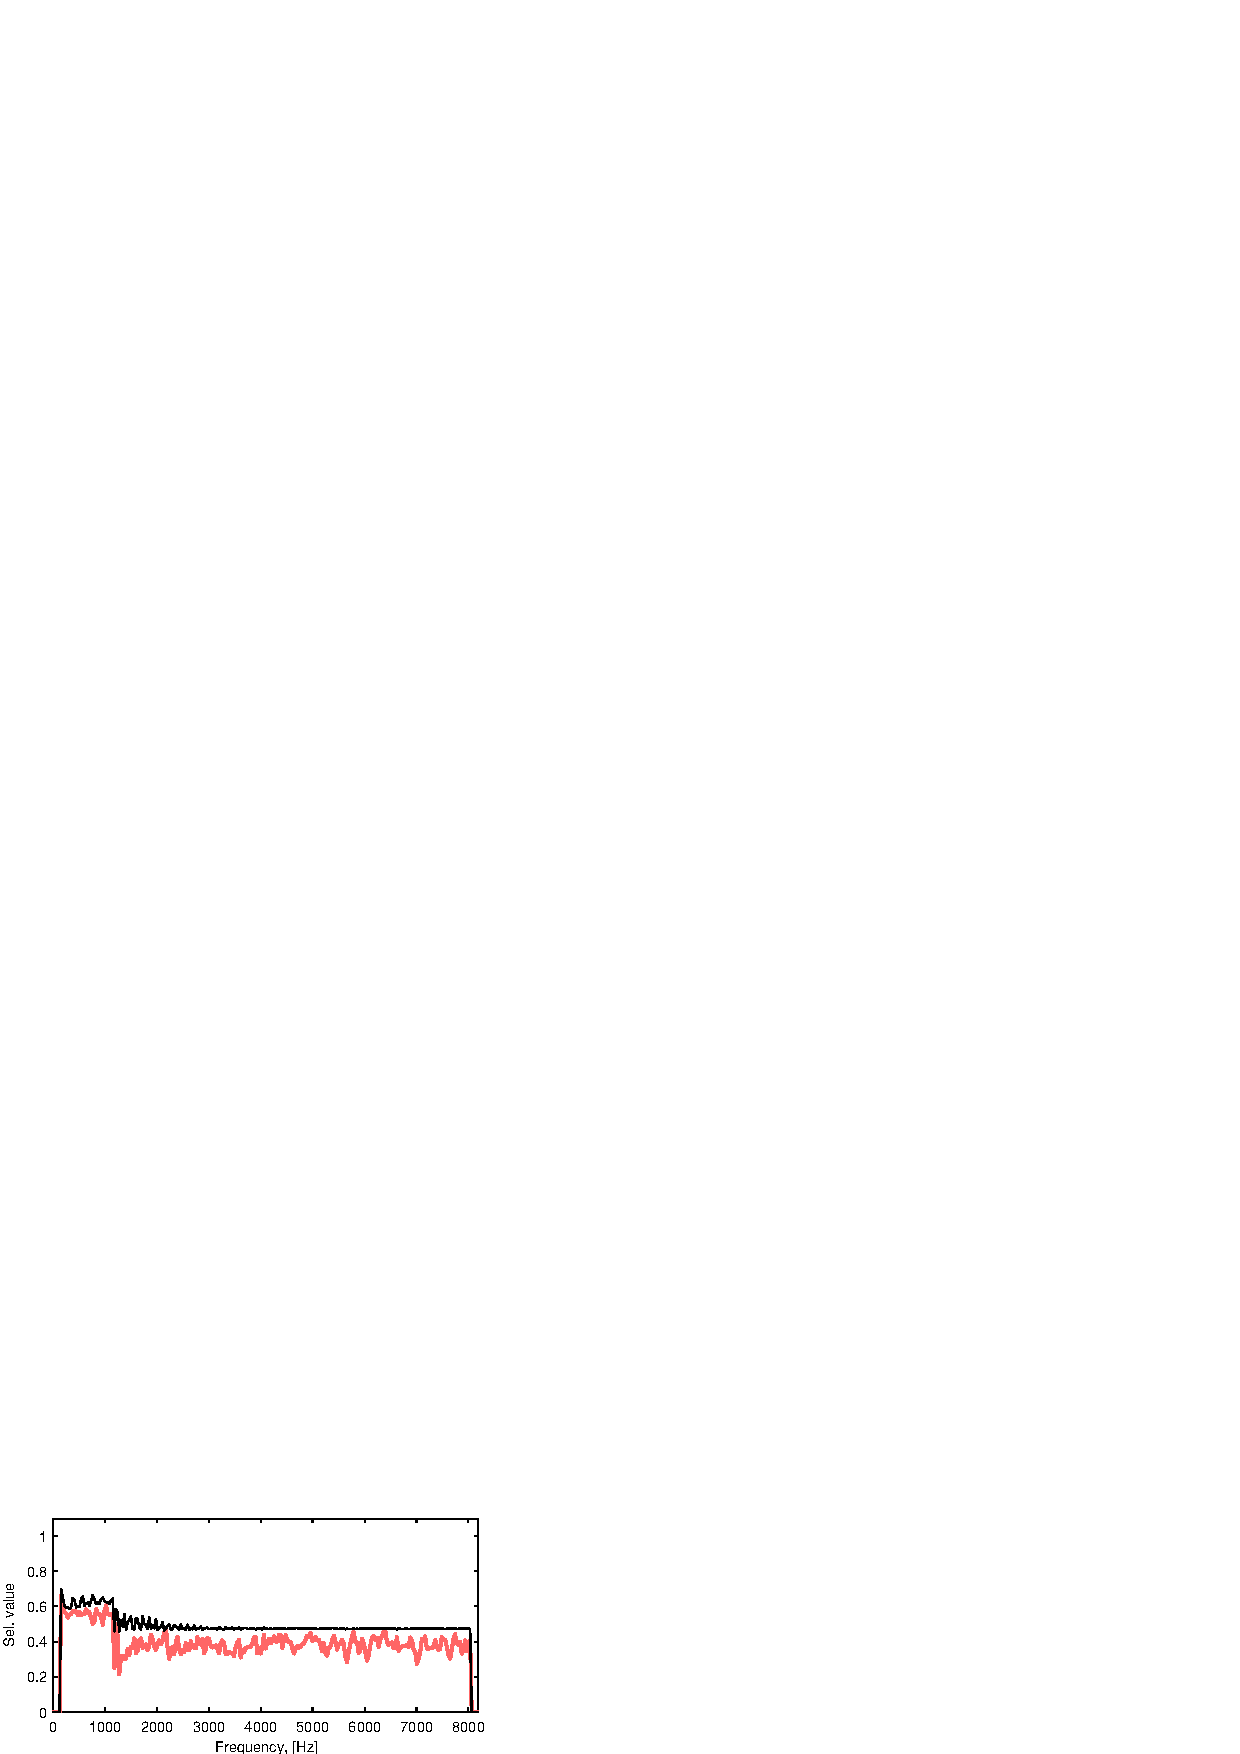
\includegraphics[width=0.49\textwidth]{methodology/filtering/sin_const-quantile_99_g}
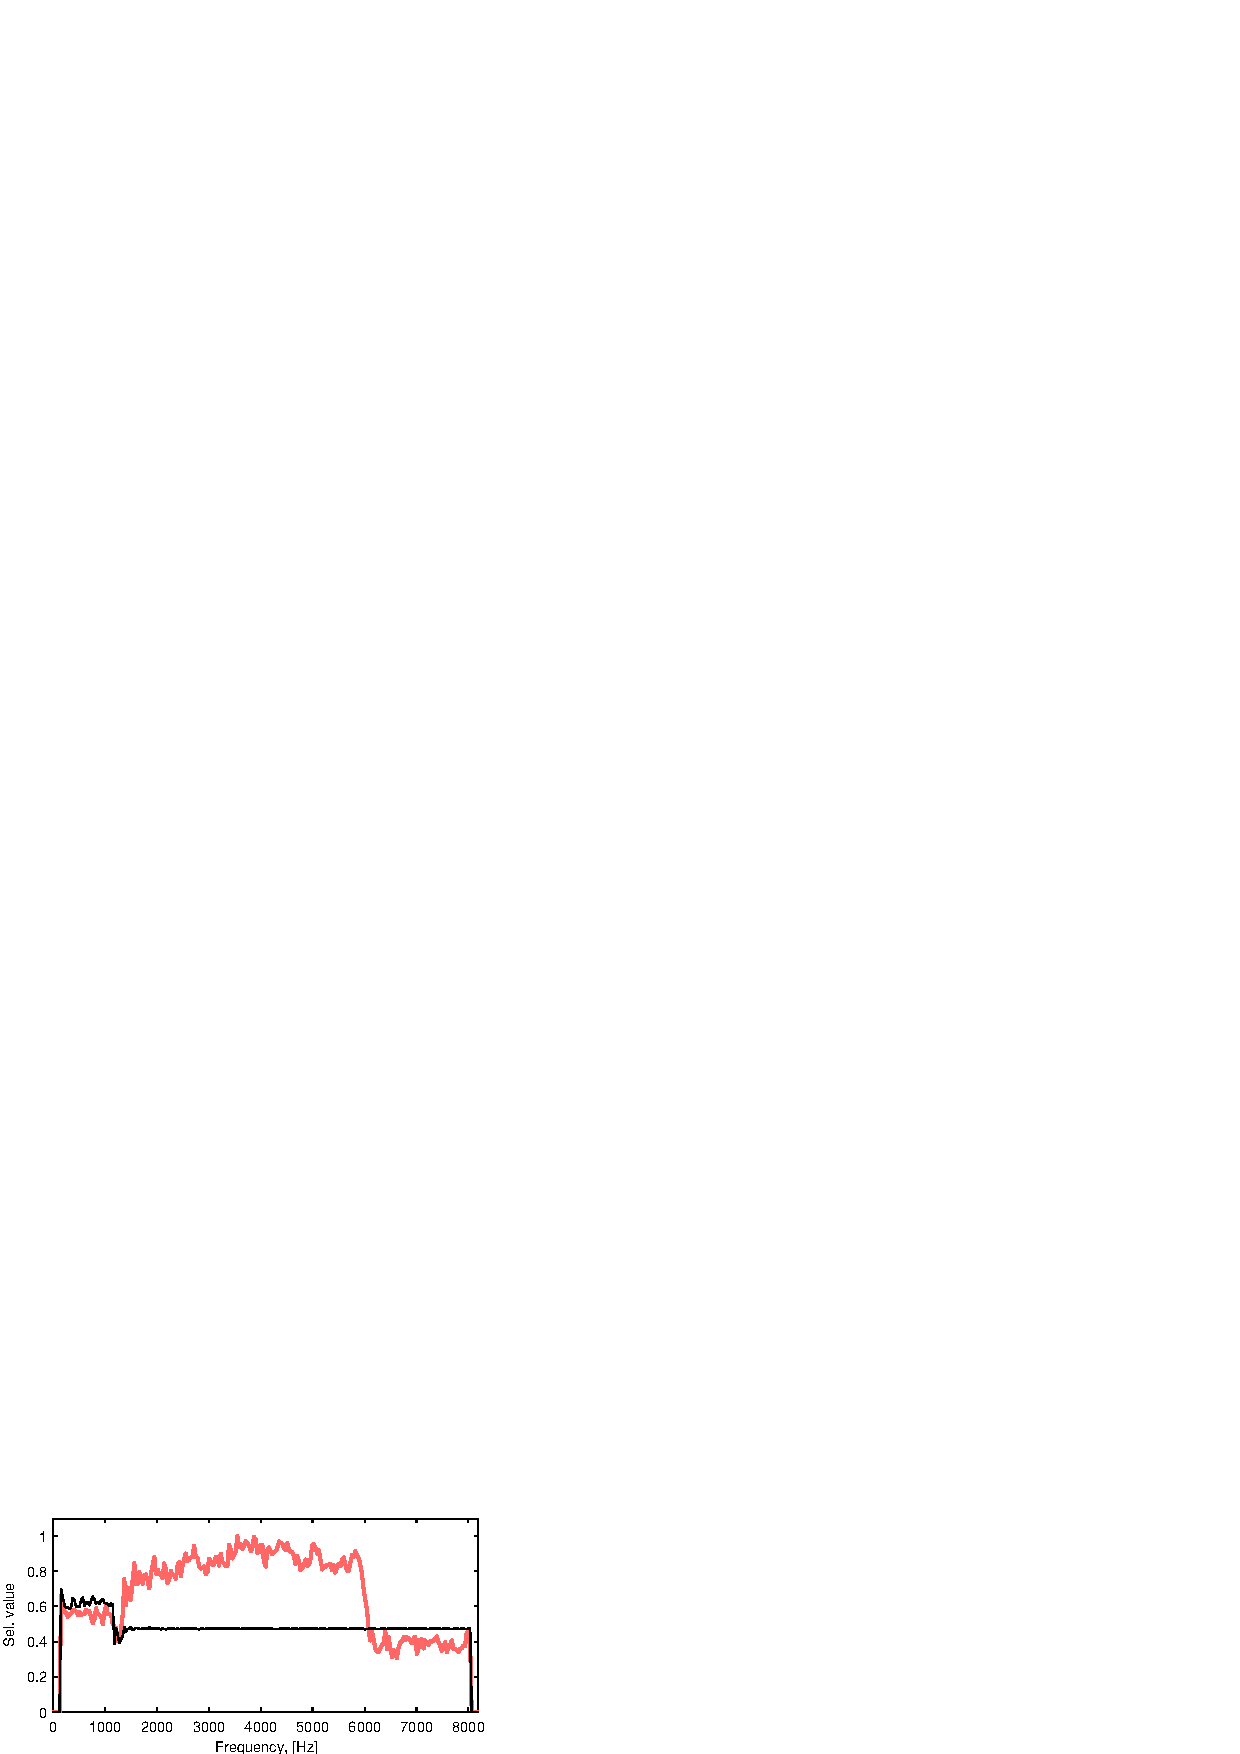
\includegraphics[width=0.49\textwidth]{methodology/filtering/sin_const-quantile_99_b}
\caption{Selector values of reference signals. Faulty (right panels) and healthy machine (left panels). Red thick lines represent selector values based on $H_{aver}$. Top panels present quantile lines of orders: 0.1, 0.3, 0.5, 0.7 and 0.9 (black thin lines) obtained upon selector values of 1000 reference signals. Bottom panels present significance thresholds for the selector values, i.e. quantile of order 0.99. Note that only at a few frequency bins selector values for healthy machine exceeds the threshold and the threshold is significantly exceeded at 2000-7000~Hz for faulty machine.\label{filtering_sim-selekt}}
\end{center}
\end{figure}
This step is essential when energy contained in the informative frequency band is relatively low, i.e. the signal also contains high-energy components that do not carry information about the local damage. In order to illustrate this point, consider a vibration signal that consists of: a) high-energy low-frequency component (component related to normal operation of the machine), b) low-energy component located at the half of the frequency range (component related to local damage) and c) low-energy noise located at the highest frequency bands (non-informative from diagnostic point of view). Values of any selector (that indicates impulsivity) at low frequency bands (not related to damage) are significantly lower than selector values at middle frequency bands (related to local damage). Thus, the signal filtered using such selector might still be affected by the low-frequency component. In other words, high spectral amplitudes of low-frequency signal components multiplied by low selector values might be still larger than low amplitudes (located at informative, middle frequency bands) multiplied by a high values of the selector. Thus, the whole procedure might provide unsatisfactory results, i.e. energy of non-informative components will dominate in the filtered signal.\\
Another reason describing benefits of thresholding is derived from analysis of a signal that consists of the high-energy low-frequency component and the noise only. It might happen that selector values at low frequency bands, containing high-energy  deterministic content, are different from values at frequency bands containing noise (with relatively low energy). Such case might be caused by specific windowing, e.g. when the STFT window length is not large enough to appropriately estimate energy flow at low frequency bands. Fig.~\ref{filtering_sim-selekt} illustrates this point. The signals $r_1(t)$ and $r_2(t)$ presented therein are sums of 6 sine waves with frequencies $190n$~Hz, $n=1,\ldots,6$ and a noise dependent on whether the signal from faulty or healthy machine is simulated. The signals $\left\{r_k(t)\right\},\,k=1,2$ are obtained using the following formula:
\begin{eqnarray}
r_k(t)=\sum^{N}_{n=1}{ A a_n \sin(2\pi f_n t)} + \sigma m_k(t),
\end{eqnarray}
where $N=6$, $A=10$, $a_n=0.75^{(n-1)}$, $f_n=190n$, $\sigma=0.1$ and $\left\{m_k(t)\right\},\,k=1,2$ is the noise. The signal from a healthy machine corresponds to the noise $m_1(t)$, which basically is a zero-mean white Gaussian noise with standard deviation equal to 1. $m_2(t)$ is related to a faulty machine and structure of this signal is more complicated. In order to construct $m_2(t)$ we decompose the signal $m_1(t)$ by filtering into 3 components: a) $\left\{m_{1a}(t)\right\}$ - low-pass filtered $\left\{m_1(t)\right\}$ with cut-off frequency 2000~Hz, b) $\left\{m_{1b}(t)\right\}$ - bandpass filtered $\left\{m_1(t)\right\}$ with cut-off frequencies 2000~Hz and 7000~Hz and c) $\left\{m_{1c}(t)\right\}$ - high-pass filtered $\left\{m_1(t)\right\}$ with cut-off frequency 7000~Hz. We use ideal filters, i.e. filters with characteristics equal to 1 along the passed band and 0 elsewhere. Then, we modulate amplitude of $\left\{m_{1b}(t)\right\}$ using an impulsive signal - sum of 128 sine waves with frequencies that are multiples of the fault frequency - $13$~Hz. As a result, the amplitude of the signal between impulses becomes similar to the corresponding amplitude of $\left\{m_1(t)\right\}$. Signal to noise ratio defined as $\mathrm{SNR_{dB}} = 10 \log_{10} \left ( \frac{P_\mathrm{signal}}{P_\mathrm{noise}} \right )$, where $P_\mathrm{signal}$ denotes power of $\sigma m_k(t)$ and $P_\mathrm{noise}$ - power of $\sum^{N}_{n=1}{ A a_n \sin(2\pi f_n t)}$, equals to -42.53~dB in healthy case ($m_1(t)$) and -36.21~dB in faulty case ($m_2(t)$). Frequency sampling is $16384$~Hz and length of the signals is $2.5$~s. The time-frequency map that provides sub-signals is calculated using 133-sample-long Kaiser windows ($\beta=5$) and discrete Fourier transform calculated in 512 points. It can be noticed that values of $H_{aver}$ at low frequency bands are different than values of $H_{aver}$ at middle and high frequency bands. Thus, we claim that each single frequency bin should be thresholded individually.\\
The proposed thresholding procedure is inspired by so called "pre-whitening". Pre-whitening is a method that flattens frequency spectrum of the examined signal~\cite{Sawalhi2005231,Sawalhi2011549,Sawalhi2011846}. Formula for the pre-whitened version of a signal $x(t)$ is~\cite{Borghesani2013370}:
\begin{equation}
y(t)=IDFT\left\{\frac{DFT\left(x(t)\right)}{\left|DFT\left(x(t)\right)\right|}\right\},
\end{equation}
where $DFT$ and $IDFT$  indicate the discrete Fourier transform and its inverse. Frequency spectrum of a signal processed using pre-whitening is flat, but the signal might still contain spikes related to local damage. When the damage signature is weak, the pre-whitened signal might be dominated by noise from frequency bands outside the informative frequency band. Thus, there is a need for enhancement of the pre-whitened signal.\\
We use an inverse of pre-whitening in order to simulate a large number of signals without transients (so called reference signals), but keeping the amplitude spectrum similar to the real data's frequency spectrum. Basically, we multiply absolute value of discrete Fourier transform of the examined signal (e.g. $r_k(t)$ or real data) element-wise by discrete Fourier transform of white noise, i.e. $DFT\left\{n(t)\right\}$, where $n(t)$ is a vector of independent identically distributed Gaussian random variables with mean $\mu=0$ and variance $\sigma^2=1$. Length of $n(t)$ is the same as length of the examined signal. Then, we return to time domain using inverse discrete Fourier transform. The formula for a simulated signal without transients is:
\begin{equation}
s(t)=IDFT\left\{{\left|DFT\left(p(t)\right)\right|}{DFT\left(n(t)\right)}\right\},
\end{equation}
where $p(t)$ is the examined signal and the multiplication is performed element by element. Next, we calculate values of the selector for each reference signal $s(t)$.\\
The procedure is repeated with a lot (e.g. 1000) of different $n(t)$'s (so called Monte Carlo method), thus we obtain a significant number of selector values for each frequency bin. Finally, a certain quantile (e.g. $99\%$) is calculated individually for every $f$. If the selector value at $f$ is lower than the quantile, it is said to be insignificant and set to 0. Otherwise, only the excess over the quantile is taken for final design of the filter.\\
Fig.~\ref{filtering_coloring-stft} in Sec.~\ref{results_filtering_real_data} presents a spectrogram of a vibration signal from a locally damaged heavy rotating machine (a two-stage gearbox from a mining company) and a spectrogram of an exemplary realization of the simulated signal $s(t)$. One can see that both signals share similar content along frequency axis, but the simulated one has no wide-band excitations related to local damage.
\subsection{Filtering}
In the final step we propose to follow the approach presented in~\cite{Combet2009652}, where the optimal Wiener filter based on the $SK$ is described. Recall, that the filter is proportional to the square root of the $SK$. We propose to follow this approach to the selectors proposed in Sec.~\ref{filtering_selectors} and replace square root of the $SK$ by square root of selector values that remains after filter's amplitude response enhancement (thresholding). We also normalize these square roots by their maxima in order to make visual comparison of them easier.\\
Firstly, the discrete Fourier transform of the examined signal is calculated and the filter's amplitude response obtained in Sec.~\ref{filtering_thresholding} is interpolated at all the frequency bins of the discrete Fourier transform. Next, the discrete Fourier transform is multiplied element-wise by the interpolated frequency characteristic. Finally, the inverse discrete Fourier transform is used in order to return to the time domain. The formula for the filtered signal $z(t)$ is as follows:
\begin{equation}
z(t)=IFT\left\{{FT\left(x(t)\right)}{W(f)}\right\},
\end{equation}
where $W(f)$ is the amplitude response of the filter driven by a given selector (e.g. $SK(f)$, $KSS(f)$, $H_{aver}(f)$, etc.), i.e. square root of thresholded values of the selector, interpolated to make the size of $W(f)$ equal to the size of discrete Fourier transform of $x(t)$.
\FloatBarrier
\subsection{Discussion}\label{methodology_filtering_discussion}

In this section we discuss motivation and properties of the proposed methodology and compare it with existing methods. The novelty of the paper is contained mainly in the extension of SK-based filtering (including the thresholding procedure), thus we discuss other methods of one dimensional clustering that might be found in the literature. One dimensional methods of clustering are significantly different from multidimensional ones. The 1D real-valued data is only a special case of multidimensional data, but the difference is in natural ordering of real numbers. All of the discussed methods benefit from this property. The fundamental problem is to distinguish between significant and insignificant values of a particular selector. Thus, there is a need for clustering values of the selector into two groups only.\\
The classical approach for filtering based on the spectral kurtosis (calculated from the STFT) is to subtract 2 from calculated fourth-order statistic and then take only excess over a given significance level $\alpha$, which is proportional to the given quantile of the normal distribution~\cite{Combet2009652,Antoni2006308}. While applying other impulsivity criteria (selectors) to the signal, one can derive analogous thresholds for each single selector. On the other hand, one can simply exploit one of the existing 1D thresholding procedures. We recall and analyze only a few of them, because comparing thresholding methods is not the goal of this paper.\\
In 1979 N. Otsu proposed a method for finding the threshold that minimizes the variance within the group, namely a weighted sum of each group's variances, where weights are just the number of elements in a particular group divided by the number of all thresholded values~\cite{Otsu197962}. In order to calculate this variance-minimizing threshold it is proposed to calculate firstly the variance within the group, taking as the threshold each element of the entire set in the sequence. Then, the final threshold is the argument which minimizes the variance within the group. In our case, where the entire set of selector values is denoted by $\left\{W(f),\,f\in \left\{ 1,\ldots,F\right\}\right\}$ it is only needed to calculate, for each $f_i\in \left\{ 1,\ldots,F\right\}$, the weighted average of variances of each of two groups - one constituted from elements of $\left\{W(f)\leq W\left(f_i\right),\,f\in \left\{ 1,\ldots,F\right\}\right\}$  and $\left\{W(f) > W\left(f_i\right),\,f\in \left\{ 1,\ldots,F\right\}\right\}$. Then, $f_i$ that maximized the weighted sum of variances is the final threshold. Such method is known for setting the threshold close to the component with larger class probability or larger class variance~\cite{Hou20061732}, thus it might fail if only a small frequency band is non-informative (with low values of $W(f)$) and values of $W(f)$ at other frequency bands are much higher and scattered. Then, the threshold might be too high, what results in ignoring some of the informative frequency bins. Recently, a new method for such heavy-tailed 1D data classification called "head/tail breaks" has been proposed by B. Jiang~\cite{Jiang2013482}. In order to avoid the effect of threshold shifting through the right tail of the data, it is proposed to iteratively constitute breakpoints (thresholds). Each breakpoint divides a set into two subsets - one above and one below the breakpoint. These breakpoints are just arithmetic means of the considered set, thus in the first step the arithmetic mean $\mu_1$ of all values in $\left\{W(f),\,f\in \left\{ 1,\ldots,F\right\}\right\}$ is calculated. Then, the mean $\mu_2$ of values above $\mu_1$ is calculated, and so on. In our case, where $\left\{W(f),\,f\in \left\{ 1,\ldots,F\right\}\right\}$ has to be divided into two groups only, this method might provide unsatisfactory results when, for instance, there are just a few values of the selector at IFB much higher than others therein, and low values at non-informative frequency band are present, as usual. Arithmetic mean is known to be sensitive to outliers, thus, once again, some of informative components might be omitted. To sum up, both methods are interesting since they do not assume specific distribution of the data. However, they might omit some informative components, for which corresponding values of the selector are not the largest, but still are significant. This remark led us to invent the thresholding method described in Sec.~\ref{filtering_thresholding}. This one might be applied not only to the kurtosis calculated from the spectrogram, but also to other selectors, for which taking a given quantile of Gaussian distribution is not a method proved as efficient. The only thing we assume is that the reference signal which imitates the same signal as the investigated one, but without local damage, might be simulated using the inverse pre-whitening. Using a number of such simulated signals it can be examined, whether our investigated machine significantly differs from a healthy one or not. Additional advantage of this method is its insensitivity to windowing, i.e. when a particular STFT windowing method provides unlikely high values of a selector for some frequency bands, the method adapts and makes the threshold higher at these bands. One can also make the procedure closer to the reality, i.e. when an appropriate (large) number of signals representing the same measurement related to a healthy machine, might be acquired. Since this extension might be performed well in a laboratory, its application to an industrial case might be difficult.
\FloatBarrier

\section{Blind equalization}\label{methodology_equalization}
Consider an input signal $\varepsilon,\,n=1,\ldots,N$ (raw vibration signal). The classical version of the minimum entropy deconvolution is based on searching for coefficients $f_l,\, l=1,\ldots,L$ of a filter which maximizes the following objective function of the filter's output $y_n$~\cite{Wiggins197821}:
\begin{equation}
O_4\left(f\left[l\right]\right)=\frac{\sum\limits_{n=1}^{N} y^4[n]}{\left[\sum\limits_{n=1}^{N} y^2[n]\right]^2},
\label{equalization_KURTOSIScriterion}
\end{equation}
where $y_n=\sum\limits_{l=1}^{L} f[l]\varepsilon [n-l]$. Optimal coefficients of the filter are calculated by solving
\begin{equation}
\frac{\partial \left(O_4\left(f\left[l\right]\right)\right)}{\partial \left(f[l]\right)}=0.
\label{equalization_derivative_zero}
\end{equation}
Since $\frac{\partial y[n]}{\partial f[l]}=\varepsilon[n-l]$, Eq.~(\ref{equalization_derivative_zero}) can be rewritten as:
\begin{equation}
\frac{\sum\limits_{n=1}^{N} y^2[n]}{\sum\limits_{n=1}^{N} y^4[n]}\sum\limits_{n=1}^{N} y^3[n]\varepsilon[n-l]=\sum\limits_{p=1}^{L} f[p] \sum\limits_{n=1}^{N} \varepsilon[n-p]\varepsilon[n-l].
\label{equalization_derivative_final_kurtosis}
\end{equation}
Denoting the left side of Eq.~(\ref{equalization_derivative_final_kurtosis}) as $b$ (cross correlation of the input and the output cubed) and the right side of Eq.~(\ref{equalization_derivative_final_kurtosis}) as multiplication of the vector $f$ and the Toeplitz autocorrelation matrix $A$, Eq.~(\ref{equalization_derivative_final_kurtosis}) can be expressed as $b=fA$ (matrix form of Eq.~(\ref{equalization_derivative_final_kurtosis})). This system might be solved iteratively. A clear description of the iterative procedure might be found in~\cite{Wiggins197821,Endo2007906}. In the literature one can find many different criteria that define the moment to stop iterations. For instance, the iterative procedure might be stopped while a minimum change in objective function of the filter's output is reached~\cite{McDonald2012237}, while correlation coefficient between outputs related to two following iterations is close enough to 1~\cite{Broadhead2000885} or while difference between filter coefficients related to two following iterations is small enough~\cite{Endo2007906}. In this paper we analyze behavior of several stopping criteria through a fixed number of iterations.\\
The combined skewness-kurtosis criterion that we analyze in this paper is based on the Jarque-Bera (JB) statistic. The JB statistic calculated for the output signal $y_n,\,n=1,\ldots,N$ is defined as~\cite{Jarque1980255}:
\begin{eqnarray}\label{equalization_eq:4}
JB(y)=\frac{N}{6}\left(S(y)^2+\frac{\left(K(y)-3\right)^2}{4}\right),
\end{eqnarray}
where $S(y)$ and $K(y)$ are the skewness and kurtosis of the output, respectively. The JB statistic is sensitive to both skewness and excess kurtosis - any deviation from zero skewness and zero excess kurtosis increases the JB statistic. Such statistical properties are profitable especially when the blind equalization algorithm with JB statistic as the cost function is applied to a vibration signal which is leptokurtic, skew or both. The JB statistic is a special case of the LM (Lagrange multiplier) statistic used in the so-called “score test”, known also as the Lagrange multiplier test. The score test can be used for testing a general class of distributions with given density function. Under the $H_0$ hypothesis, namely the vector of observations constitutes sample from some specific distribution, the LM statistic has asymptotically $\chi ^2$ distribution with $r$ degrees of freedom ($r$ - number of parameters of this distribution). The JB statistic is a particular case of LM statistic for Gaussian distribution. In our case the asymptotic distribution of JB defined as in Eq.~(\ref{equalization_eq:4}) is $\chi ^2$ with 2 degrees of freedom (as the number of parameters in Gaussian distribution).  It is worth mentioning that the test based on skewness and kurtosis is locally most powerful when the test statistic has form as in Eq.~(\ref{equalization_eq:4}). For more details see~\cite{Jarque1987163}. The asymptotic distribution of JB statistic (defined as in Eq.~(\ref{equalization_eq:4})) is also discussed in~\cite{Bai200549}.\\
On the basis of the JB statistic we propose the following objective function for blind equalization algorithm:
\begin{equation}
O_{JB}\left(f\left[l\right]\right)=\left(\frac{\frac{1}{N}\sum\limits_{n=1}^{N} y^3[n]}{\left[\frac{1}{N}\sum\limits_{n=1}^{N} y^2[n]\right]^{\frac{3}{2}}}\right)^2 + \frac{1}{4}\left(\frac{\frac{1}{N}\sum\limits_{n=1}^{N} y^4[n]}{\left[\frac{1}{N}\sum\limits_{n=1}^{N} y^2[n]\right]^2}-3\right)^2.
\label{equalization_JBcriterion}
\end{equation}
Calculating $f$ for which:
\begin{equation}
\frac{\partial \left(O_{JB}\left(f\left[l\right]\right)\right)}{\partial \left(f[l]\right)}=0
\label{equalization_derivative_zero_JB}
\end{equation}
one can obtain filter coefficients for which the optimization criterion defined in Eq.~(\ref{equalization_JBcriterion}) is maximized.\\
Thus, the analogous formula to Eq.~(\ref{equalization_derivative_final_kurtosis}) is:
\begin{equation}
\frac{C_{1}\sum\limits_{n=1}^{N} y^2[n]\varepsilon[n-l]+C_{2}\sum\limits_{n=1}^{N} y^3[n]\varepsilon[n-l]}{C_3} = \sum\limits_{p=1}^{L} f[p] \sum\limits_{n=1}^{N} \varepsilon[n-p]\varepsilon[n-l],
\label{equalization_derivative_final_JB}
\end{equation}
where:
\begin{equation}
\begin{split}
C_1& =3\frac{1}{N}\sum\limits_{n=1}^{N} y^3 \left(\frac{1}{N}\sum\limits_{n=1}^{N} y^2\right)^2\\
C_2& =\frac{1}{N}\sum\limits_{n=1}^{N} y^4 \frac{1}{N}\sum\limits_{n=1}^{N} y^2-3\left(\frac{1}{N}\sum\limits_{n=1}^{N} y^2\right)^3\\
C_3& =3\left(\frac{1}{N}\sum\limits_{n=1}^{N} y^3\right)^2 \frac{1}{N}\sum\limits_{n=1}^{N} y^2-3\frac{1}{N}\sum\limits_{n=1}^{N} y^4 \left(\frac{1}{N}\sum\limits_{n=1}^{N} y^2\right)^2.
\end{split}\label{equalization_derivative_final_const}
\end{equation}
Similarly as in Eq.~(\ref{equalization_derivative_final_kurtosis}), the left side of Eq.~(\ref{equalization_derivative_final_JB}) consists of weighted cross correlations and the right side is a multiplication of  the vector $f$ and the Toeplitz autocorrelation matrix $A$. The filter $f$ has to be normalized (by its Euclidean norm) in every iteration to control energy of the filter's output, thus Eq.~(\ref{equalization_derivative_final_JB}) can be simplified. i.e. dividing by $C_3$ is not necessary. $\frac{1}{N}\sum\limits_{n=1}^{N} y^k$ is the $k$-th order moment and $\sum\limits_{n=1}^{N} y^k[n]\varepsilon[n-l]$ is the cross correlation of the input and the output to the power $k$. Eq.~(\ref{equalization_derivative_final_JB}) might be solved for $f$ using the standard iterative algorithm described in~\cite{Wiggins197821}. As it is mentioned in~\cite{Ooe1979458}, the recommended way of calculating cross correlations is based on the Wiener-Khinchin theorem, i.e. using the Fast Fourier Transform (FFT) and its inverse (IFFT). Benefits from using FFT and IFFT are clearly perceptible when the order of the filter is large and the input signal is long.\\
In order to provide comprehensive analysis, we compare the results obtained using kurtosis and JB statistic as criteria with the blind deconvolution driven by one of Gray's variability norms, that incorporates normalized third statistical moment (skewness). The objective function is defined as~\cite{Gray1979}:
\begin{equation}
O_3\left(f\left[l\right]\right)=\frac{\sum\limits_{n=1}^{N} y^3[n]}{\left[\sum\limits_{n=1}^{N} y^2[n]\right]^\frac{3}{2}},
\label{equalization_SKEWNESScriterion}
\end{equation}
where $y_n=\sum\limits_{l=1}^{L} f[l]\varepsilon [n-l]$. Optimal coefficients of the filter are calculated by solving
\begin{equation}
\frac{\partial \left(O_3\left(f\left[l\right]\right)\right)}{\partial \left(f[l]\right)}=0.
\label{equalization_derivative_zeroSKEW}
\end{equation}
Eq.~(\ref{equalization_derivative_zeroSKEW}) can be rewritten as:
\begin{equation}
\frac{\sum\limits_{n=1}^{N} y^2[n]}{\sum\limits_{n=1}^{N} \left| y\right|^3[n]}\sum\limits_{n=1}^{N}\left|y\right|^3[n]\varepsilon[n-l]=\sum\limits_{p=1}^{L} f[p] \sum\limits_{n=1}^{N} \varepsilon[n-p]\varepsilon[n-l].
\label{equalization_derivative_final_SKEW}
\end{equation}
The left side of Eq.~(\ref{equalization_derivative_final_SKEW}) consists of weighted cross correlation and the right side is a multiplication of  the vector $f$ and the Toeplitz autocorrelation matrix $A$. The iterative algorithm mentioned earlier solves Eq.~(\ref{equalization_derivative_final_SKEW}) for $f$.


\section{Autoregressive model in case of multiple damage}\label{methodology_twostage}

The proposed two-stage procedure is based on signal filtering. Here we use both autoregressive modeling and optimal frequency band selection. Sometimes, the raw vibration signal contains a strong deterministic contamination which is highly amplitude modulated. In such case of time varying signal-to-noise ratio the signal of interest is invisible in both time series and envelope spectrum. Then, signal filtering based on measures of dispersion (e.g. the spectral kurtosis) may indicate a wrong frequency band as informative. We propose to filter out the deterministic signal using autoregressive filtering. The next step is based on linear filtering using frequency characteristics of the filter obtained by measures of impulsiveness. We compare filters driven by the spectral kurtosis~\cite{Combet2009652} and one of informative frequency band selectors presented in~\cite{Obuchowski2013441,Obuchowski2013,Obuchowski2014138}.
As it was mentioned, we use the autoregressive model to filter out highly amplitude modulated mesh harmonics. The AR model of order $p$ is defined as follows:
\begin{equation}
\sum_{i=0}^p\phi(i)X(t-i)=\epsilon(t),
\end{equation}
where $\phi(0)=0$ and $\epsilon(t)$ stands for noise.\\
It is known, that the AR time series model is able to model noisy sinusoidal pattern if its characteristic polynomial has complex roots. In the case of a large number of harmonics a high-order AR model is expected with at least two complex roots corresponding to one mesh harmonic. As the optimal order indicator we use the highest Kolmogorov-Smirnov criterion, i.e. $\mathrm{AR}(p)$ is said to be optimal if the Kolmogorov-Smirnov (KS) test statistic of residuals is the highest~\cite{Zhan20071953}. According to the fact that the residual signal in case of local damage should be impulsive, it is expected that the distance between empirical distribution and Gaussian one is high – the higher KS statistic, the more impulsive signal. Recall the KS statistic for signal $X(t)$ is defined as follows~\cite{Justel1997251}:
\begin{equation}
KS=\sup{x}\left|\hat{F}(x)-F(x)\right|,
\end{equation}
where $\hat{F}(x)$ is the empirical cumulative distribution function for given signal while $F(x)$ is the cumulative distribution function of Gaussian distribution with parameters estimated form the signal.\\
Moreover, the results of AR filtering are also checked by comparing time-frequency maps of the residual signal with the raw signal. Parameters of the AR model are obtained by using Yule-Walker~\cite{Brockwell1991}.
Fig.~\ref{twostage_fig01}
\begin{figure}[ht]
\begin{center}
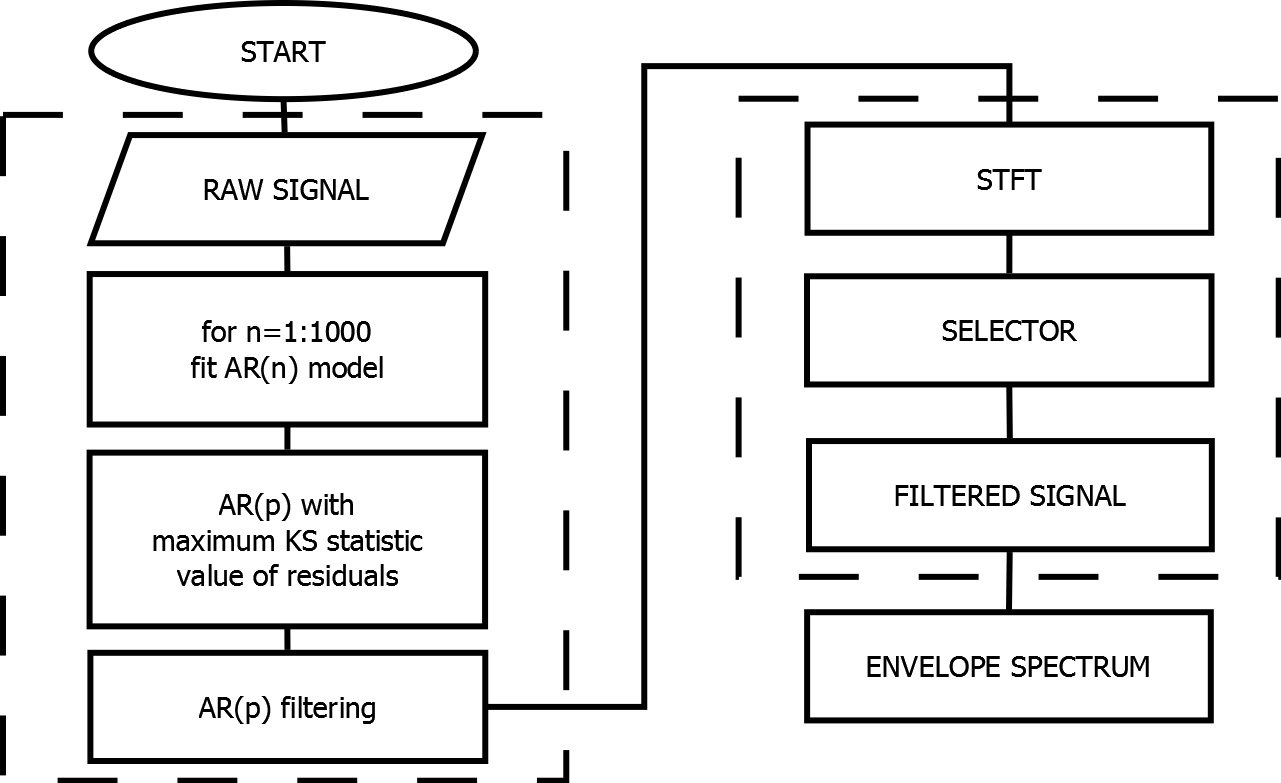
\includegraphics[width=0.7\textwidth]{methodology/twostage/twostage_diagram}
\caption{Block diagram of the two-stage procedure}\label{twostage_fig01}
\end{center}
\end{figure}
Once mesh harmonics are suppressed during the previous step of the procedure, the residual signal might be still noisy, e.g. when the SOI is relatively narrowband. We propose to select the informative frequency band using the average horizontal distance on quantile-quantile plot (QQplot)~\cite{Obuchowski2013441,Obuchowski2013,Obuchowski2014138}. Namely, we quantify the average distance between markers and reference line on the QQplot. The QQplot we use here is a graphical goodness-of-fit tool which compares quantiles of empirical distribution of the sample with the Gaussian distribution. The reference line connects first and third quartiles of both distributions. We compare it to the well-known spectral kurtosis. Both of them are based on analysis of narrowband slices of a time-frequency map. In this paper we design the filter using not only the characteristic given by a selector but we also enhance the characteristic by using individual thresholds of selector's value for a given frequency bin. Namely, we put 0 in the frequency characteristic of the filter if the value of the selector is lower than the threshold for a given frequency bin. The thresholds are obtained using the Monte Carlo method and inverse pre-whitening~\cite{Obuchowski2013}.\\
After designing the filter, we filter out the residual signal by computing Fourier transform of the signal, multiplying it by frequency response of the selector-based filter and, finally, using the inverse Fourier transform to return to the time domain. This method is an extension of the method presented in~\cite{Combet2009652}, where the filter is constructed using the spectral kurtosis.\\
A block diagram of our two-stage procedure is presented in Fig.~\ref{twostage_fig01}.
\FloatBarrier

\section{Periodic autoregressive model for cyclic load of bucket wheel excavator}\label{methodology_par}

\subsection{Influence of non-Gaussian noise to PAR estimation}

The signals analyzed in this section is represent vibration acceleration of a planetary gearbox used in a bucket wheel excavator~\cite{dybala2014empirical}. - \hl{NO TO TRZEBA JAKOS INACZEJ UJAC} Such vibration signal might be simulated as a sum of several sinusoidal components with frequencies that meet the gear mesh frequency and its harmonics and a white noise. Due to the cyclic regime in which the excavator operates, the sinusoidal components are frequency and amplitude  modulated with the period corresponding to the period of the bucket wheel operation~\cite{Chaari2012635}. Due to industrial environment, we decided to analyze white noises that follow the double Pareto distribution with parameters $\alpha_1=1.5$ (denoted later as Pareto1.5) and $\alpha_2=3.6$ (denoted as Pareto3.6) and compare result with the Gaussian case. Let us point out for $\alpha_2$ the examined Pareto distribution have finite second moment while for $\alpha_1$ the second moment does not exists. This fact has important influence for the results.\\
Influence of non-Gaussian noise to PAR estimation is performed using the following algorithm. At first, a lot of signals related to each type of noise are simulated to preserve reliability of results. Energy of each noise sequence is normalized, i.e. time series are divided by its standard deviation to preserve fair comparison. Secondly, parameters of the PAR models are estimated for each signal. The procedure of estimation is based on the Yule-Walker method and is described in~\cite{Wylomanska2014171}. Order of the PAR model is chosen as 15 for every signal. This choice is motivated by the number of sinusoidal components and the fact, that the residual time series are satisfactory~\cite{Wylomanska2014171}. After that, we analyze amplitude response of the models at each $1\leq t \leq T$, namely a surface of amplitude response. It is a natural extension of the amplitude response of an autoregressive model. The autoregressive model (AR) of order $p$ and parameters $a=(a_i)_{i=1,\ldots,p}$ is defined as follows:
\begin{eqnarray}
X(t)-\sum^{p}_{i=1}a_i X(t-i)=Z(t),
\end{eqnarray}
where the sequence ${Z(t)}$ is a white noise time series.\\
Amplitude response of an autoregressive model with coefficients $a=(a_i)_{i=1,\ldots,p}$ is defined as follows:
\begin{eqnarray}
S(f)=\left|\frac{1}{FT(a)}\right|,
\end{eqnarray}
where $FT(a)$ is the discrete Fourier transform (DFT) of $a=(a_i)_{i=1,\ldots,p}$. The amplitude response of an autoregressive model is a tool used for interpretation of its coefficients. It illustrates how the model applied to an input signal increases amplitudes of input’s spectral components. For an autoregressive model with time-varying coefficients a natural extension of the amplitude response is a surface of amplitude response. Therefore it depends not only on the frequency $f$, but on the time instance $t$, as well. Thus, the surface of amplitude response is defined as:
\begin{eqnarray}
S(t,f)=\left|\frac{1}{FT\left(a(t)\right)}\right|,
\end{eqnarray}
Interpretation of the surface of amplitude response is similar to the classical, one dimensional amplitude response, i.e. $S(t,f)$ describes how the model applied to an input signal increases amplitudes of input's spectral components at the time instance $t$.\\
In order to examine influence of the considered distribution to PAR model estimation we calculate the mean square error (MSE) between estimated amplitude response and so called "perfect surface", described in \hl{Sec. 4.2}. To preserve fair results, every surface (estimated and "perfect") is normalized by its average value, i.e. arithmetic mean of the whole surface is subtracted from the surface. Higher MSE means that the procedure gives worse results in the considered case.
\FloatBarrier

\subsection{Influence  to PAR estimation for different number of period repetitions}

In this section we analyze influence of the number of period repetitions on PAR parameters estimation procedure. Such analysis is motivated by the question how long the data acquisition should be to ensure appropriate results using the PAR model. In order to examine influence of different number of period replications we analyze MSE between PAR parameters ${a_i(t)}_i=1,\ldots,p,\, t=1,\ldots,T$ estimated from the noiseless signals and corresponding noisy signals of different numbers of period repetitions. The minimum number of period repetitions is set to 3 and the maximum - to 18. We compare boxplots and medians to clearly see how the estimation procedure is influenced by the number of period repetitions.

\FloatBarrier


\section{Conclusions}


Podsumowanie rezultatow?